% % ===============================
% \subsection{Nguồn 3: Billboard Hot 100}
% \subsubsection{Giới thiệu dữ liệu}
    
%     \textbf{Bối cảnh} \\
    
%     - Từ năm 2025, Spotify đã ngừng công khai dữ liệu bảng xếp hạng \textbf{Global Top 200} hằng tuần. Điều này khiến việc thu thập dữ liệu gốc phục vụ cho phân tích trở nên khó khăn nếu chỉ dựa vào nguồn chính thức từ Spotify. \\
    
%     - Để khắc phục hạn chế này, nhóm lựa chọn sử dụng \textbf{Billboard Hot 100} 
%     làm nguồn dữ liệu thay thế. Đây là bảng xếp hạng uy tín, được cập nhật hằng tuần vào Chủ Nhật, phản ánh mức độ phổ biến của các ca khúc trên thị trường âm nhạc \textbf{Mỹ} và có sức ảnh hưởng toàn cầu. \\
    
%     \textbf{Dữ liệu thu thập ban đầu} \\
    
%     - Pipeline được xây dựng bằng Python, sử dụng thư viện \texttt{billboard} để tự động tải danh sách \textbf{Top 100 ca khúc mỗi tuần trong năm 2025}. \\
    
%     - Các trường thông tin thu được gồm:
%     \begin{itemize}
%         \item \texttt{week}: ngày Chủ Nhật của tuần (chuẩn hóa mốc thời gian).
%         \item \texttt{rank}: thứ hạng của bài hát trong tuần.
%         \item \texttt{title}: tên bài hát.
%         \item \texttt{artist}: nghệ sĩ thể hiện chính.
%     \end{itemize}
    
%     - Bộ dữ liệu này được lưu trữ ban đầu trong tệp, làm nền tảng cho các bước \textbf{bổ sung dữ liệu (enrichment)} ở giai đoạn sau. \\
    
%     \textbf{Hạn chế của dữ liệu gốc} \\
    
%     - Billboard chỉ cung cấp \textbf{thông tin xếp hạng và metadata cơ bản} (tựa đề, nghệ sĩ), chưa có định danh duy nhất để liên kết với dữ liệu ngoài. \\
    
%     - Hoàn toàn thiếu vắng \textbf{đặc trưng âm thanh (audio features)} 
%     và \textbf{thể loại (genres)} – trong khi đây lại là các yếu tố then chốt để phân tích sâu hơn về “công thức tạo hit” và “xu hướng thể loại theo thời gian”. \\

    

% % =========================
% \subsubsection{Thu thập và bổ sung dữ liệu }

% \textbf{Giải pháp từng bước} 

% \begin{enumerate}
%     \item \textbf{Thu thập Billboard Hot 100}
%     \begin{itemize}
%         \item Sinh danh sách ngày Chủ Nhật trong năm 2025 và tải dữ liệu xếp hạng Hot 100 cho từng tuần. 
%         \item \textbf{Kết quả:} dữ liệu gốc đã có thứ hạng bài hát theo tuần nhưng chưa đủ thông tin để phân tích chuyên sâu.
%     \end{itemize}

%     \item \textbf{Tìm Spotify track ID}
%     \begin{itemize}
%         \item Với mỗi cặp \texttt{(title, artist)} từ Billboard, gọi \textbf{Spotify Search API} để tìm \texttt{spotify\_id}. 
%         \item  \textbf{Kết quả:} bổ sung khóa định danh duy nhất giúp liên kết với các API khác.
%     \end{itemize}

%     \item \textbf{Lấy audio features từ ReccoBeats}
%     \begin{itemize}
%         \item Gọi \textbf{ReccoBeats API} để lấy các đặc trưng âm nhạc: \texttt{danceability, energy, tempo, valence, speechiness, acousticness, instrumentalness, liveness, loudness, key, mode}.
%         \item Do API giới hạn batch, pipeline được thiết kế để chia nhỏ các request (\texttt{BATCH\_SIZE = 30}). 
%         \item \textbf{Kết quả:} dataset đã mô tả được ``chất âm'' của từng bài hát.
%     \end{itemize}

%     \item \textbf{Lấy genres từ Spotify API}
%     \begin{itemize}
%         \item Sử dụng \texttt{spotify\_id} để gọi endpoint \texttt{track/artist} nhằm lấy thể loại (genres) của nghệ sĩ chính.
%         \item Nếu genres trống thì gán \texttt{NaN}.
%         \item  \textbf{Kết quả:} dataset cuối cùng đã có thêm nhãn \textbf{thể loại âm nhạc} cho từng ca khúc.
%     \end{itemize}


    
% \end{enumerate}


% % ==========================
%     \subsubsection{Phân tích dữ liệu ban đầu}
    
%     \textbf{Lý do} 
    
%     - Sau khi đã bổ sung dữ liệu từ nhiều nguồn khác nhau, cần tiến hành phân tích dữ liệu ban đầu (Exploratory Data Analysis – EDA) 
%     để hiểu rõ cấu trúc, chất lượng cũng như các vấn đề tiềm ẩn trước khi bước vào giai đoạn làm sạch và trích xuất đặc trưng. \\
    
%     \textbf{Giải pháp} 
    
%     \begin{enumerate}[label=\arabic*]
%         \item \textbf{Tổng quan dữ liệu}
%         \begin{itemize}
%             \item Thống kê số dòng, số cột, tên các trường dữ liệu.
%             \item Kiểm tra kiểu dữ liệu, số lượng giá trị bị thiếu (Null), số dòng trùng lặp.
%             \item Tính toán các thống kê mô tả cơ bản cho dữ liệu số.
%     \end{itemize}
%      Số dòng: 3900, Số cột: 17
%     \begin{longtable}{|>{\raggedright\arraybackslash}p{2.8cm}|
%                           >{\raggedright\arraybackslash}p{2cm}|
%                           >{\raggedright\arraybackslash}p{6cm}|
%                           >{\raggedright\arraybackslash}p{5cm}|}
%         \hline
%         \textbf{Column} & \textbf{DataType} & \textbf{Meaning} & \textbf{How to Use} \\ \hline
%         \endfirsthead
        
%         \hline
%         \textbf{Column} & \textbf{DataType} & \textbf{Meaning} & \textbf{How to Use} \\ \hline
%         \endhead
        
%         week & object & Ngày Chủ Nhật của tuần trong BXH Billboard (YYYY-MM-DD). & Mốc thời gian để phân tích xu hướng theo tuần. \\ \hline
%         rank & int64 & Thứ hạng bài hát (1 = cao nhất, 100 = thấp nhất). & Phân tích Top 10/50, đo độ bền hạng, vẽ timeline. \\ \hline
%         title & object & Tên bài hát. & Hiển thị trên dashboard, kết hợp với week để vẽ xu hướng. \\ \hline
%         artist & object & Tên nghệ sĩ chính. & Phân tích Top Artist, số lần vào BXH, xu hướng hợp tác. \\ \hline
%         spotify\_id & object & ID duy nhất của track trên Spotify. & Làm khóa để join với Spotify API/ReccoBeats. \\ \hline
%         danceability & float64 & Mức độ dễ nhảy (0–1). & Đặc trưng hit songs, cao trong Pop/Dance. \\ \hline
%         energy & float64 & Độ “năng lượng” của bài hát (0–1). & So sánh hit vs non-hit, nhận diện nhạc sôi động. \\ \hline
%         tempo & float64 & Nhịp độ bài hát (beats per minute – BPM) & Phân tích BPM phổ biến trong các hit. \\ \hline
%         valence & float64 & Mức độ tích cực/vui vẻ (0–1). & Phân biệt nhạc vui (valence cao) với ballad (thấp). \\ \hline
%         speechiness & float64 & Mức độ giọng nói (0–1). & Cao trong Rap/Hip-hop, thấp trong Pop/Ballad. \\ \hline
%         acousticness & float64 & Mức độ acoustic (0–1). & Ballad/Indie cao; Pop/EDM thấp. \\ \hline
%         instrumentalness & float64 & Khả năng là nhạc không lời (0–1). & EDM/nhạc nền cao, Pop vocal thấp. \\ \hline
%         liveness & float64 & Mức độ biểu diễn live (0–1). & Phát hiện bài hát thu live concert. \\ \hline
%         loudness & float64 & Độ lớn trung bình (dB). & Kết hợp với energy để phân tích phong cách sản xuất. \\ \hline
%         key & float64 & Tông nhạc (0–11). & Phân tích xu hướng tông nhạc ưa chuộng. \\ \hline
%         mode & float64 & Thang âm: 1=Major, 0=Minor. & So sánh mood Major vs Minor. \\ \hline
%         genre & object & Thể loại chính (Spotify API). & Nhóm xu hướng theo genre, Top genres theo rank/streams. \\ \hline
        
%         \caption{Bảng mô tả dữ liệu }
%         \label{tab:data_dictionary}
%         \end{longtable}
    

%     \item \textbf{Trực quan giá trị thiếu}
%      \begin{itemize}
%         \item Vẽ heatmap để quan sát sự phân bố các giá trị bị thiếu theo cột.
%         \item Nhận diện các cột thiếu dữ liệu nhiều, cần xử lý trong bước làm sạch.
%     \end{itemize}
    
%     \begin{figure}[H] % dùng [H] để giữ hình tại đúng vị trí (cần \usepackage{float})
%         \centering
%         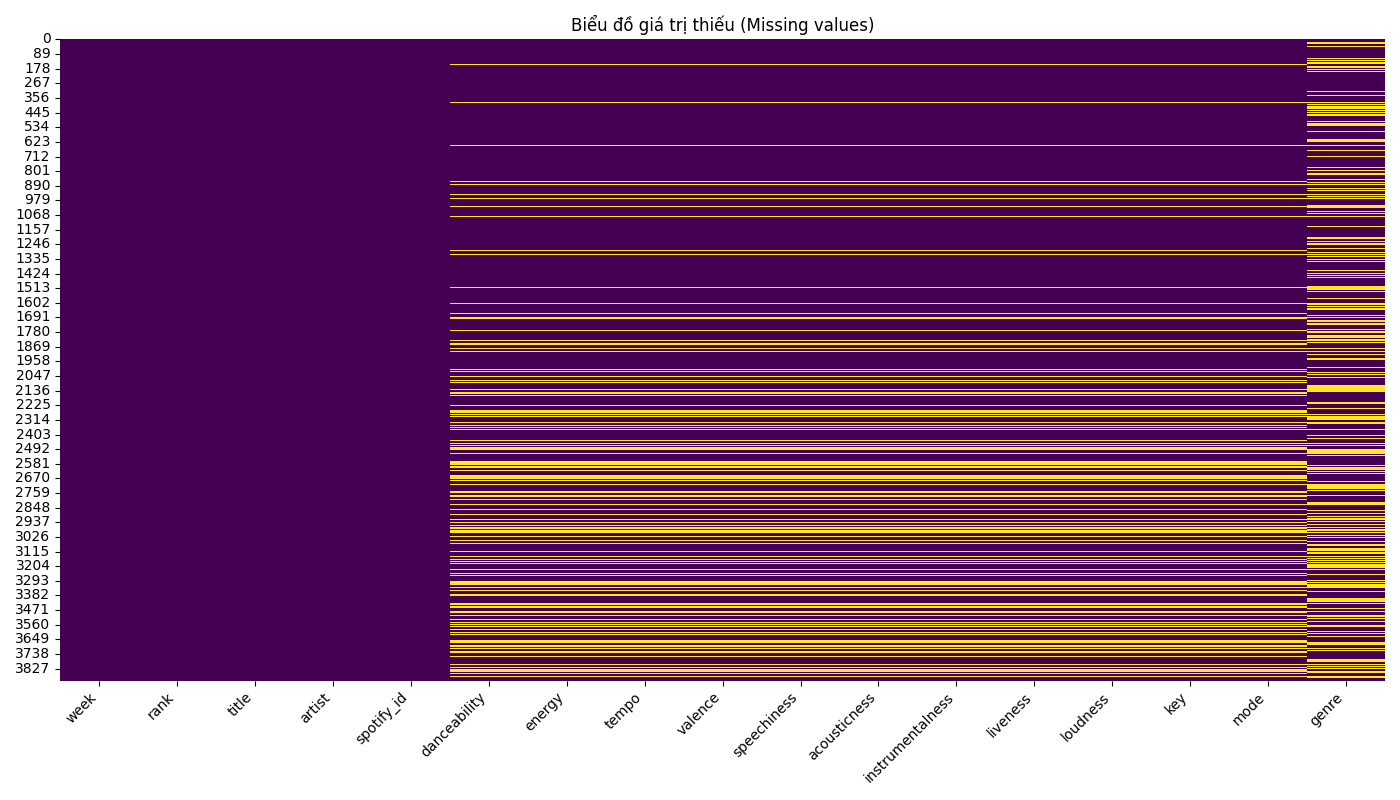
\includegraphics[width=1.0\textwidth]{../graphics/data3/Output/step1/missing_values.png}
%         \caption{Biểu đồ heatmap thể hiện các giá trị thiếu trong dữ liệu}
%         \label{fig:missing}
%     \end{figure}
%     Biểu đồ heatmap trên cho thấy một số cột dữ liệu xuất hiện nhiều giá trị thiếu (các vạch sáng). Cụ thể, các trường liên quan đến \texttt{audio features} (như \texttt{danceability}, \texttt{energy}, \texttt{tempo}, \texttt{valence}, \texttt{speechiness}, \texttt{acousticness}, \texttt{instrumentalness}, \texttt{liveness}, \texttt{loudness}) và trường \texttt{genre} có tỷ lệ thiếu khá cao. Điều này xuất phát từ việc Billboard chỉ cung cấp dữ liệu thứ hạng, tên bài hát và nghệ sĩ, trong khi các đặc trưng âm nhạc và thể loại phải được bổ sung từ API ngoài.  Việc trực quan hóa bằng heatmap giúp nhận diện nhanh các cột còn thiếu nhiều giá trị,từ đó đưa ra chiến lược xử lý hợp lý trong bước làm sạch dữ liệu.

%     \item \textbf{Phân bố các thuộc tính âm nhạc}
%     \begin{itemize}
%         \item Vẽ histogram kèm KDE cho các thuộc tính quan trọng: \texttt{danceability}, \texttt{energy}, \texttt{tempo}, \texttt{valence}, 
%         \texttt{speechiness}, \texttt{acousticness}, \texttt{instrumentalness}, \texttt{liveness}, \texttt{loudness}.
%         \item Giúp hiểu rõ phân phối của từng đặc trưng.
        
%          \begin{figure}[H] % dùng [H] để giữ hình tại đúng vị trí (cần \usepackage{float})
%             \centering
%             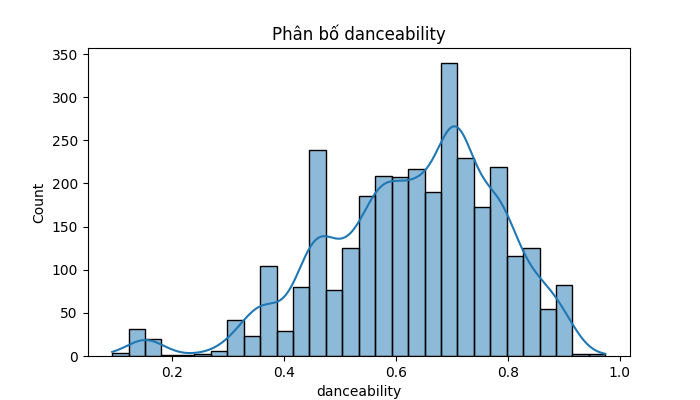
\includegraphics[width=1.0\textwidth]{../graphics/data3/Output/step1/danceability_distribution.png}
%             \caption{Biểu đồ phân bố \texttt{danceability} của các bài hát.}
%             \label{fig:missing}
%         \end{figure}
%     Biểu đồ trên cho thấy đa số các bài hát có giá trị \texttt{danceability} tập trung trong khoảng 0.5 -- 0.8. Điều này phản ánh rằng các ca khúc phổ biến trên thị trường âm nhạc toàn cầu thường có tiết tấu dễ nhảy, phù hợp với thị hiếu nghe nhạc của công chúng. Những bài hát có \texttt{danceability} quá thấp hoặc quá cao chỉ chiếm tỷ lệ nhỏ, cho thấy thị trường ưu tiên sự cân bằng giữa khả năng nhảy và tính giai điệu.
        
%     \end{itemize}

%     \item \textbf{Phân bố thể loại âm nhạc}
%     \begin{itemize}
%         \item Loại bỏ nhãn \texttt{NaN}, sau đó thống kê tần suất xuất hiện của các thể loại.
%     \end{itemize}

%     \begin{figure}[H] % dùng [H] để giữ hình tại đúng vị trí (cần \usepackage{float})
%             \centering
%             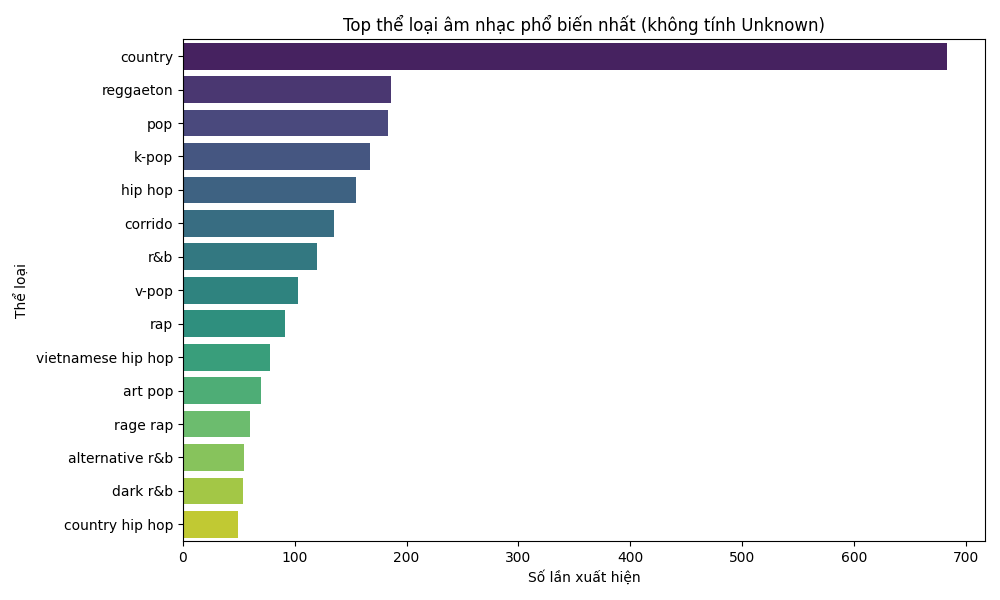
\includegraphics[width=1.0\textwidth]{../graphics/data3/Output/step1/genre_distribution.png}
%             \caption{Top 15 thể loại âm nhạc phổ biến nhất .}
%             \label{fig:missing}
%     \end{figure}
%     Biểu đồ trên cho thấy thể loại \textbf{Country} chiếm ưu thế vượt trội với gần 700 lần xuất hiện, cao hơn hẳn so với các thể loại còn lại. Các dòng nhạc như \textbf{Reggaeton}, \textbf{Pop}, \textbf{K-pop}, \textbf{Hip Hop} cũng nằm trong nhóm dẫn đầu, phản ánh xu hướng toàn cầu hiện nay. Đáng chú ý, \textbf{V-Pop} và \textbf{Vietnamese Hip Hop} cũng có sự hiện diện nhất định, cho thấy nhạc Việt đang dần khẳng định vị thế trong thị trường quốc tế. Sự phân bố này gợi ý rằng các doanh nghiệp và nghệ sĩ có thể ưu tiên đầu tư vào các thể loại đang thịnh hành như Country, Pop hay K-pop để tối ưu cơ hội tiếp cận khán giả rộng hơn.

%     \item \textbf{Ma trận tương quan}
%     \begin{itemize}
%         \item Tính hệ số tương quan giữa các biến số.
%         \item Phát hiện mối quan hệ mạnh.
%         \begin{figure}[H] % dùng [H] để giữ hình tại đúng vị trí (cần \usepackage{float})
%             \centering
%             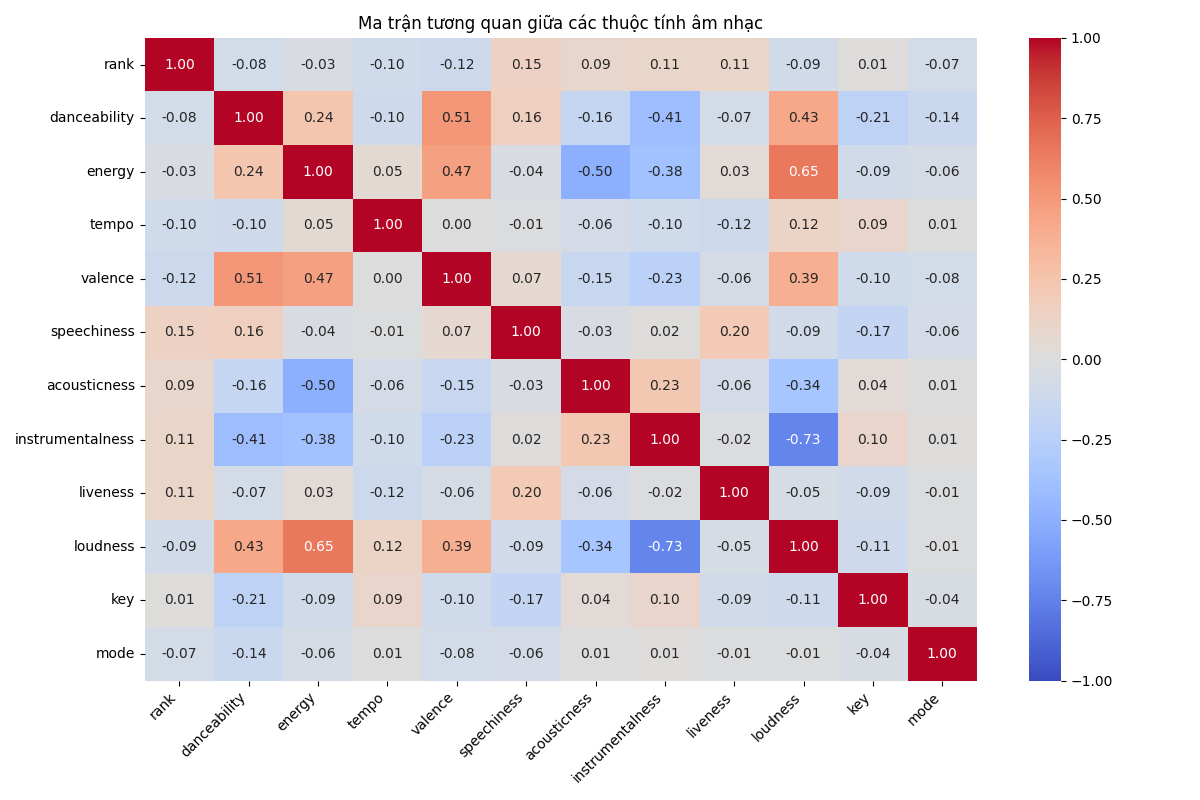
\includegraphics[width=1.0\textwidth]{../graphics/data3/Output/step1/correlation_matrix.png}
%             \caption{Ma trận tương quan giữa các thuộc tính âm nhạc.}
%             \label{fig:missing}
%         \end{figure}
%     Biểu đồ trên cho thấy một số mối quan hệ nổi bật giữa các đặc trưng âm nhạc. \textbf{Energy} có tương quan dương mạnh với \textbf{Loudness} (0.65), phản ánh rằng các bài hát có cường độ năng lượng cao thường đi kèm với âm lượng lớn. Ngược lại, \textbf{Acousticness} có tương quan âm với \textbf{Energy} (-0.50), cho thấy nhạc acoustic thường có mức năng lượng thấp. \textbf{Danceability} và \textbf{Valence} cũng có mối quan hệ dương (0.51), gợi ý rằng những ca khúc dễ nhảy thường mang lại cảm xúc tích cực. Những phát hiện này hỗ trợ việc lý giải tại sao một số thuộc tính đóng vai trò quan trọng trong việc tạo nên “công thức” của các bài hit toàn cầu.
%     \end{itemize}
% \end{enumerate}

% \textbf{Kết quả / Ý nghĩa} 

% \begin{itemize}
%     \item Bộ dữ liệu đã được mô tả đầy đủ về cấu trúc và chất lượng, cung cấp cái nhìn tổng quan cần thiết trước khi làm sạch.
%     \item Phát hiện được những vấn đề cần xử lý trong bước kế tiếp (missing values, dữ liệu trùng lặp, định dạng chưa thống nhất).
%     \item Các insight sơ bộ: nhạc dễ nhảy (danceability) chiếm ưu thế, energy và loudness cao, acousticness thấp; 
%     streams có quan hệ nghịch mạnh với rank. Đây là cơ sở định hướng cho bước làm sạch dữ liệu và xây dựng đặc trưng.
% \end{itemize}
% % =========================
% \subsubsection{Làm sạch dữ liệu (Data Cleaning)}

% \textbf{Lý do} \\

% - Sau khi phân tích dữ liệu ban đầu mặc dù không có giá trị trùng lặp,nhưng nhận thấy còn tồn tại nhiều giá trị thiếu (missing values), một số cột chưa đúng kiểu dữ liệu.
% - Nếu không xử lý, các vấn đề này sẽ gây sai lệch cho kết quả phân tích và trực quan hóa ở các bước tiếp theo. \\

% \textbf{Giải pháp} \\

% \begin{enumerate}[label=\arabic*]
%     \item \textbf{Chuẩn hóa kiểu dữ liệu}
%     \begin{itemize}
%         \item Cột \texttt{week} được chuyển về định dạng \texttt{datetime}.
%         \item Cột \texttt{rank} được ép kiểu về số nguyên \texttt{Int64}.
%     \end{itemize}

%     \item \textbf{Xử lý missing values}
%     \begin{itemize}
%         \item Với các cột số (\texttt{danceability}, \texttt{energy}, \texttt{tempo}, 
%         \texttt{valence}, \texttt{speechiness}, \texttt{acousticness}, 
%         \texttt{instrumentalness}, \texttt{liveness}, \texttt{loudness}, 
%         \texttt{key}, \texttt{mode}): điền giá trị trung bình (mean).
%         \item Với cột \texttt{genre}: điền giá trị mặc định là \texttt{Unknown} nếu bị thiếu.
%     \end{itemize}

%     \item \textbf{Đánh giá lại dữ liệu sau khi làm sạch}
%     \begin{itemize}
%         \item Sử dụng heatmap để trực quan hóa, xác nhận rằng toàn bộ giá trị thiếu đã được xử lý.
%         \begin{figure}[H] % dùng [H] để giữ hình tại đúng vị trí (cần \usepackage{float})
%             \centering
%             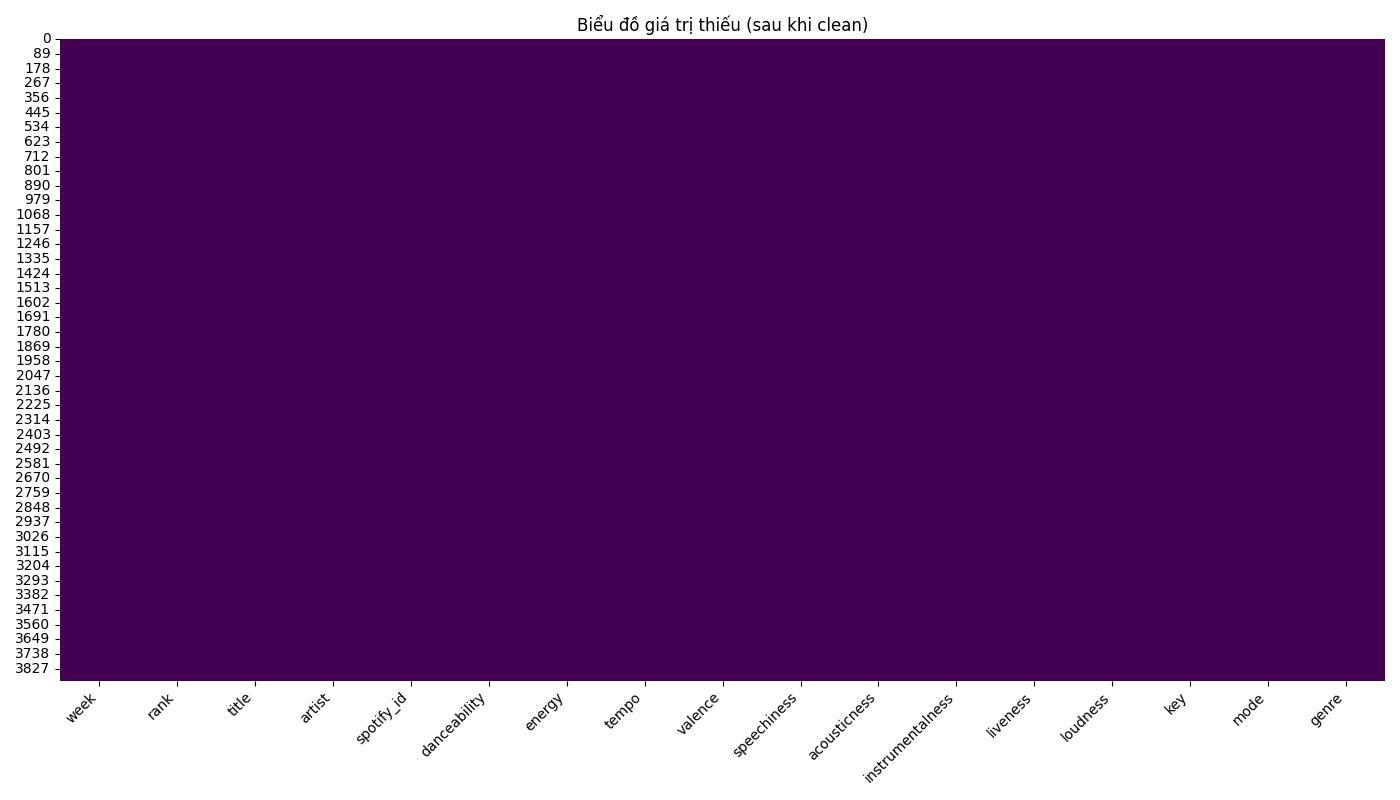
\includegraphics[width=1.0\textwidth]{../graphics/data3/Output/step2/missing_values_after_clean.png}
%             \caption{Heatmap giá trị thiếu sau khi làm sạch dữ liệu.}
%             \label{fig:missing}
%         \end{figure}
%         Biểu đồ trên cho thấy toàn bộ các cột dữ liệu đều đã được xử lý đầy đủ, 
%     không còn giá trị thiếu. Điều này chứng minh quy trình làm sạch dữ liệu đã hoàn tất, tập dữ liệu đã đồng nhất và sẵn sàng cho các bước phân tích đặc trưng và xu hướng tiếp theo.

%     \end{itemize}
% \end{enumerate}

% \textbf{Kết quả và Ý nghĩa} 

% \begin{itemize}
%     \item Bộ dữ liệu đã được chuẩn hóa và không còn giá trị thiếu.
%     \item Các cột dữ liệu quan trọng đều ở định dạng chính xác, đảm bảo độ tin cậy cho các phép phân tích.
%     \item Việc gán giá trị trung bình cho các cột số và điền \texttt{Unknown} cho thể loại 
%     giúp giữ lại toàn bộ dữ liệu, không gây mất mát bản ghi.
%     \item Dữ liệu sạch, đồng nhất, sẵn sàng cho bước tiếp theo: \textbf{Tạo đặc trưng (Feature Engineering)}.
% \end{itemize}

% % =========================
% \subsubsection{Tạo đặc trưng (Feature Engineering)}

% \textbf{Lý do} 
% - Dữ liệu sau khi làm sạch vẫn chủ yếu mô tả thông tin cơ bản như thứ hạng, nghệ sĩ và đặc trưng âm nhạc. 
% Tuy nhiên, để phân tích chuyên sâu hơn, cần có các biến phản ánh mức độ bền vững của bài hát trên BXH, 
% đặc điểm nghệ sĩ (solo/hợp tác), cũng như yếu tố thời gian (mùa trong năm). 
% - Việc tạo thêm đặc trưng mới sẽ giúp khám phá xu hướng ẩn và nâng cao giá trị phân tích. \\

% \textbf{Giải pháp} 
% \begin{enumerate}[label=\arabic*]
%     \item \textbf{Đặc trưng theo bài hát (Track-level features)}
%     \begin{itemize}
%         \item \texttt{weeks\_on\_chart\_total}: tổng số tuần xuất hiện trên BXH.
%         \item \texttt{weeks\_on\_chart\_cum}: số tuần tích lũy đến thời điểm hiện tại.
%         \item \texttt{peak\_rank}: thứ hạng cao nhất mà bài hát đạt được.
%         \item \texttt{avg\_rank}: thứ hạng trung bình của bài hát.
%         \item \texttt{is\_top10}: 1 nếu bài hát lọt Top 10 trong tuần, ngược lại là 0.
%         \item \texttt{is\_new}: 1 nếu đây là tuần đầu tiên xuất hiện trên BXH, ngược lại là 0.
%     \end{itemize}

%     \item \textbf{Đặc trưng theo nghệ sĩ (Artist-based features)}
%     \begin{itemize}
%         \item \texttt{is\_collab}: 1 nếu bài hát có sự hợp tác (nhiều nghệ sĩ, có “feat.”, “\&” hoặc dấu phẩy trong tên), 
%         ngược lại là 0.
%     \end{itemize}

%     \item \textbf{Đặc trưng theo thời gian (Time-based features)}
%     \begin{itemize}
%         \item \texttt{season}: phân loại theo mùa (Spring, Summer, Fall, Winter) dựa trên tháng trong năm.
%         \item Hỗ trợ phân tích yếu tố mùa vụ ảnh hưởng đến sự phổ biến của các thể loại nhạc.
%     \end{itemize}
% \end{enumerate}

% \textbf{Kết quả và Ý nghĩa} 

% \begin{itemize}
%     \item Bộ dữ liệu sau khi thêm đặc trưng đã phản ánh đầy đủ hơn vòng đời của bài hát, đặc điểm nghệ sĩ và bối cảnh thời gian.
%     \item Các đặc trưng như \texttt{peak\_rank}, \texttt{weeks\_on\_chart\_total} giúp đo lường mức độ bền vững của hit. 
%     \item Đặc trưng \texttt{is\_collab} cho phép đánh giá vai trò của hợp tác nghệ sĩ trong việc tạo ra các ca khúc thành công.
%     \item Đặc trưng \texttt{season} mở ra khả năng phân tích tác động của mùa vụ đến xu hướng nghe nhạc.
% \end{itemize}

% \begin{figure}[H]
%     \centering
%     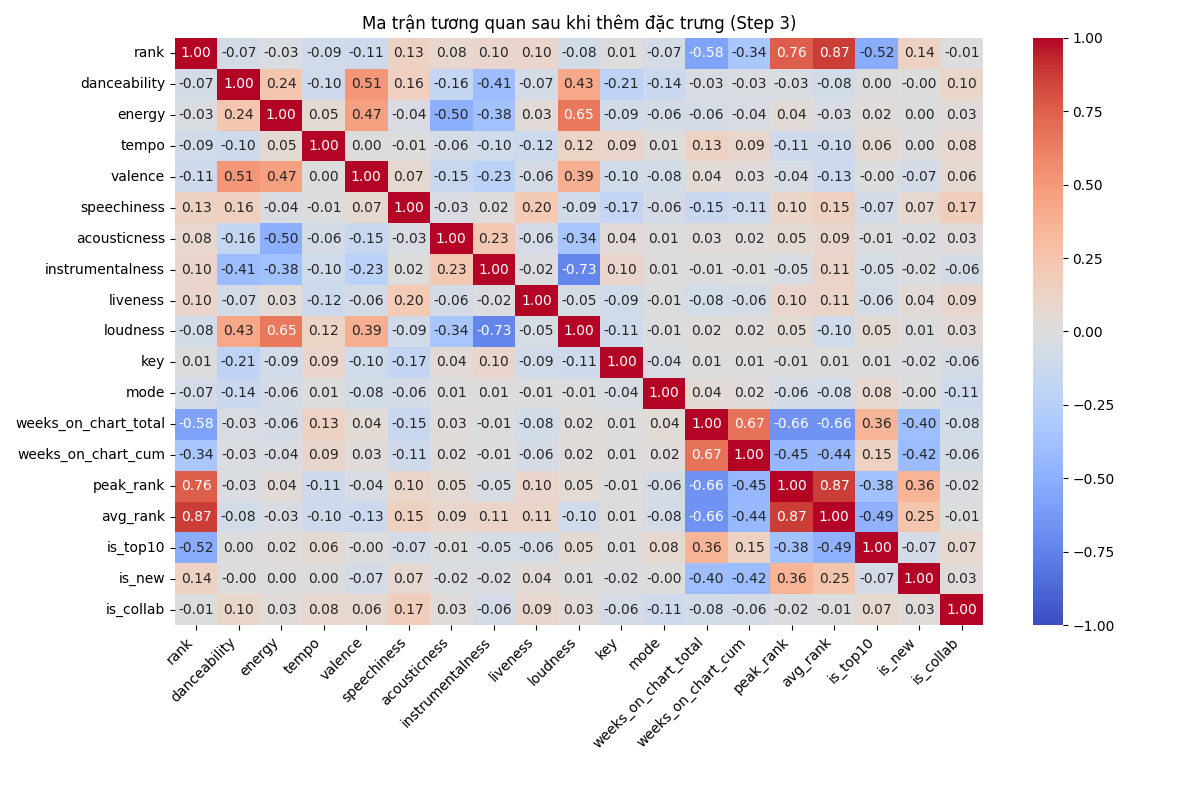
\includegraphics[width=1.0\textwidth]{../graphics/data3/Output/step3/correlation_matrix_step3.png}
%     \caption{Ma trận tương quan sau khi thêm đặc trưng}
%     \label{fig:corr_step3}
% \end{figure}

% Biểu đồ trên cho thấy các đặc trưng mới có mối quan hệ rõ rệt với các trường dữ liệu gốc: \texttt{weeks\_on\_chart\_total} và \texttt{weeks\_on\_chart\_cum} tương quan âm với \texttt{rank}, chứng tỏ các bài hát trụ hạng lâu thường có thứ hạng cao. \texttt{peak\_rank} và \texttt{avg\_rank} có tương quan mạnh với \texttt{rank}, khẳng định thứ hạng hàng tuần phản ánh hiệu suất tổng thể. 
% Đặc trưng \texttt{is\_top10} cũng có quan hệ nghịch với \texttt{rank}, 
% phù hợp với định nghĩa lọt Top 10. Trong khi đó, \texttt{is\_collab} và \texttt{is\_new} có tương quan yếu, nhưng vẫn là những yếu tố bổ sung quan trọng cho phân tích xu hướng và hành vi âm nhạc. 
% % ==========================

% \subsubsection{Phân tích xu hướng (Trend Analysis)}

% \textbf{Bối cảnh} \\

% Phần phân tích này tập trung vào dữ liệu \textbf{Billboard Hot 100 tại thị trường Mỹ năm 2025}, được bổ sung thông tin từ Spotify API và ReccoBeats. 
% Do đặc thù Billboard Hot 100 phản ánh riêng thị trường Mỹ, các insight thu được sẽ cho thấy rõ xu hướng âm nhạc chủ đạo tại Mỹ thay vì toàn cầu.

% \textbf{Lý do} \\

% - Sau khi dữ liệu đã được làm sạch và bổ sung đặc trưng, bước tiếp theo là tiến hành phân tích xu hướng. 
% - Mục tiêu nhằm phát hiện các mẫu hành vi nổi bật: cách bài hát mới xuất hiện, độ bền hit, thể loại phổ biến trong Top 10, vai trò của nghệ sĩ, yếu tố mùa vụ và mối quan hệ giữa độ bền (longevity) và vị trí cao nhất (peak rank). \\

% \textbf{Giải pháp} \\

% \begin{enumerate}[label=\arabic*]
%     \item \textbf{Xu hướng bài hát mới theo thời gian}
%     \begin{itemize}
%         \item Đếm số lượng \texttt{is\_new} theo tuần để theo dõi số lượng bài hát mới gia nhập BXH.
%         \item Trực quan bằng line chart cho thấy tuần nào có nhiều ca khúc debut nhất.
%     \end{itemize}
%     \begin{figure}[H]
%         \centering
%         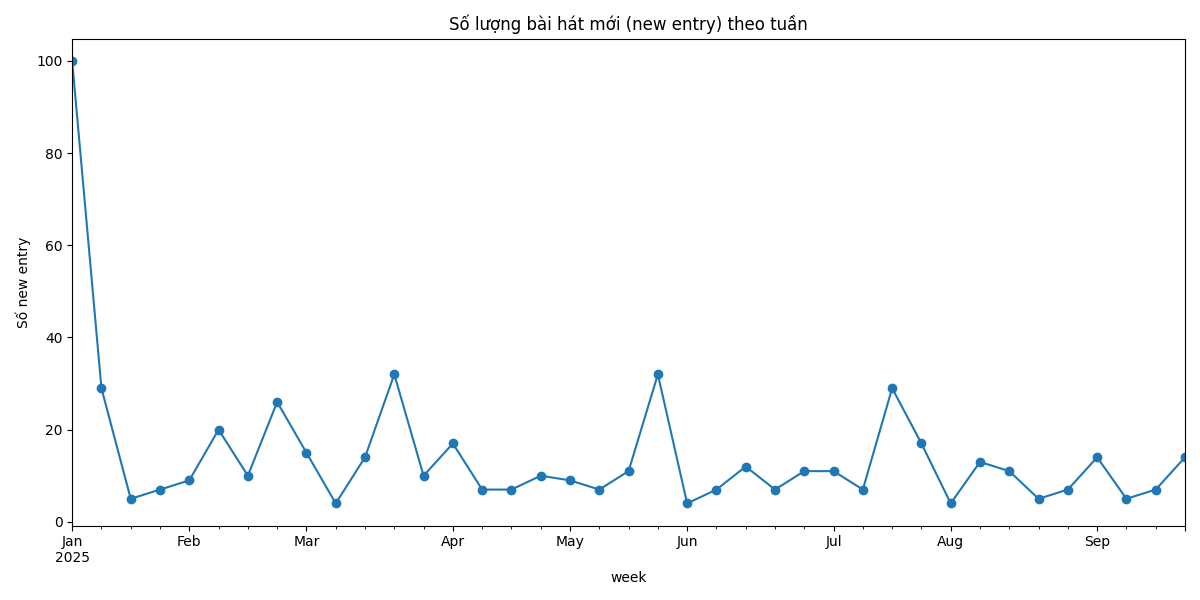
\includegraphics[width=1.0\textwidth]{../graphics/data3/Output/step4/new_entry_trend.png}
%         \caption{Số lượng bài hát mới (new entry) theo tuần trong năm 2025.}
%         \label{fig:new_entry_trend}
%     \end{figure}
%     Biểu đồ cho thấy trong tuần đầu tiên của năm 2025 có hơn 100 bài hát mới xuất hiện trên BXH Billboard Hot 100 (hiện tượng “reset” đầu năm). Sau đó, số lượng new entry giảm mạnh và dao động quanh mức 5–30 bài mỗi tuần.  Một số tuần có đột biến tăng (ví dụ cuối tháng 3, tháng 6, tháng 8), thường trùng với các đợt phát hành album lớn hoặc cao điểm mùa lễ hội. Điều này phản ánh tính cạnh tranh của thị trường âm nhạc.

%     \item \textbf{Phân phối độ bền (longevity)}
%     \begin{itemize}
%         \item Vẽ histogram số tuần một bài hát tồn tại trên BXH.
%         \item Giúp phân biệt hit “chớp nhoáng” và hit bền vững.
%     \end{itemize}
    
%     \begin{figure}[H]
%         \centering
%         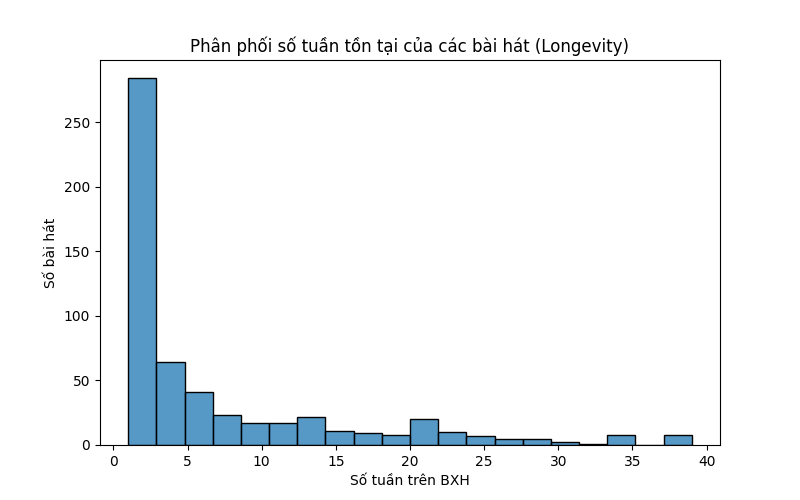
\includegraphics[width=1\textwidth]{../graphics/data3/Output/step4/hit_longevity.png}
%         \caption{Phân phối số tuần tồn tại của các bài hát trên Billboard Hot 100.}
%         \label{fig:hit_longevity}
%     \end{figure}
    
%     Biểu đồ cho thấy phần lớn các bài hát chỉ xuất hiện trên BXH trong thời gian ngắn (khoảng 1–3 tuần), phản ánh đặc trưng cạnh tranh khốc liệt của thị trường âm nhạc.  Tuy nhiên, vẫn có một nhóm nhỏ ca khúc duy trì được vị trí lâu dài (trên 20–30 tuần), được xem là những “hit bền vững” có sức hút mạnh mẽ.  
%     Kết quả này gợi ý rằng việc duy trì vị trí lâu dài trên BXH khó khăn hơn nhiều so với việc “đột phá” vào BXH ở tuần đầu tiên, và có thể phụ thuộc vào các yếu tố như độ nổi tiếng của nghệ sĩ, chiến dịch quảng bá, cũng như đặc điểm âm nhạc (energy, danceability, valence).
    

%    \item \textbf{Timeline các hit đình đám}
%     \begin{itemize}
%         \item Chọn ra một số bài có \texttt{peak\_rank = 1}, vẽ line chart thứ hạng theo thời gian.
%         \item Đảo ngược trục Y để thể hiện trực quan đường đi lên/xuống BXH.
%     \end{itemize}
    
%     \begin{figure}[H]
%         \centering
%         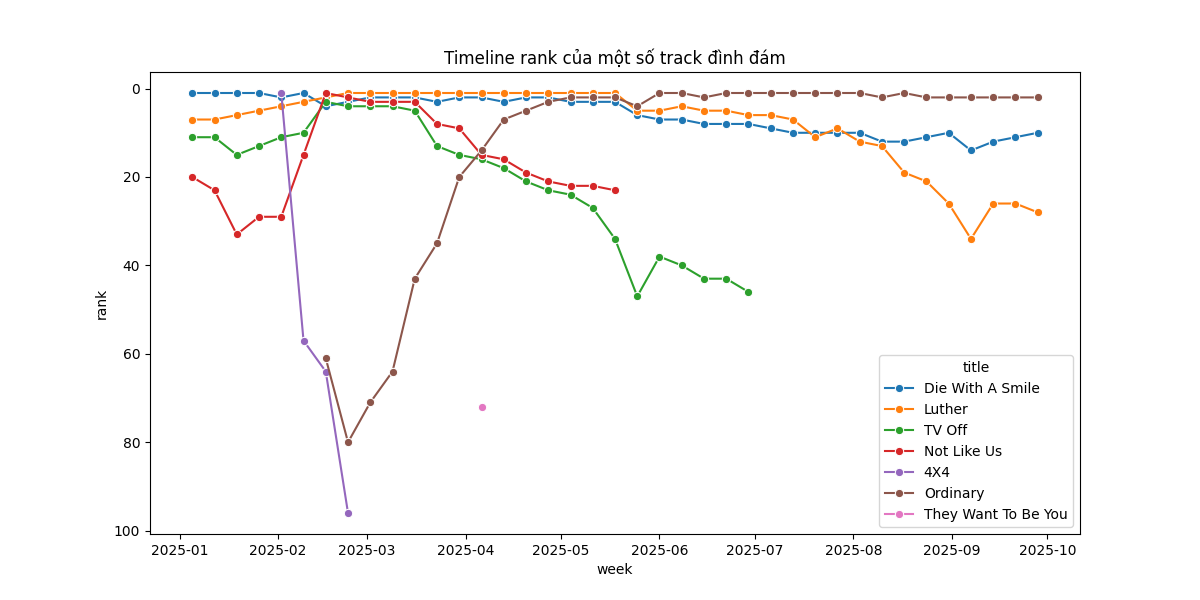
\includegraphics[width=1\textwidth]{../graphics/data3/Output/step4/track_timeline.png}
%         \caption{Timeline thứ hạng của một số ca khúc đạt vị trí số 1 trên Billboard Hot 100.}
%         \label{fig:track_timeline}
%     \end{figure}
    
%     Biểu đồ trên minh họa quá trình lên xuống hạng của một số bài hit nổi bật trong năm 2025. Có thể quan sát rằng:  
%     \begin{itemize}
%         \item Một số ca khúc như \textit{Die With A Smile}, \textit{Luther} giữ được vị trí cao trong thời gian dài, chứng tỏ sức hút ổn định và khả năng duy trì độ phổ biến.  
%         \item Các bài như \textit{TV Off}, \textit{Not Like Us} nhanh chóng leo lên Top 1 nhưng tụt hạng mạnh sau vài tuần, thể hiện đặc điểm “bùng nổ ngắn hạn”.  
%         \item Một số bài khác có quỹ đạo đi lên dần (ví dụ \textit{Ordinary}), cho thấy hiệu ứng lan tỏa muộn nhờ truyền thông hoặc viral.  
%     \end{itemize}
    
%     Điều này phản ánh sự đa dạng trong vòng đời của một hit: có ca khúc “one-hit wonder” chỉ thịnh hành trong thời gian ngắn, trong khi một số khác có khả năng trụ vững nhiều tháng liền nhờ nền tảng fanbase và chiến lược quảng bá hiệu quả.
    

%     \item \textbf{Phân tích thể loại trong Top 10}
%     \begin{itemize}
%         \item Lọc các bài có \texttt{is\_top10 = 1}, loại bỏ \texttt{Unknown}.
%         \item Đếm tần suất xuất hiện của từng thể loại → Top 10 genres.
%     \end{itemize}
    
%     \begin{figure}[H]
%         \centering
%         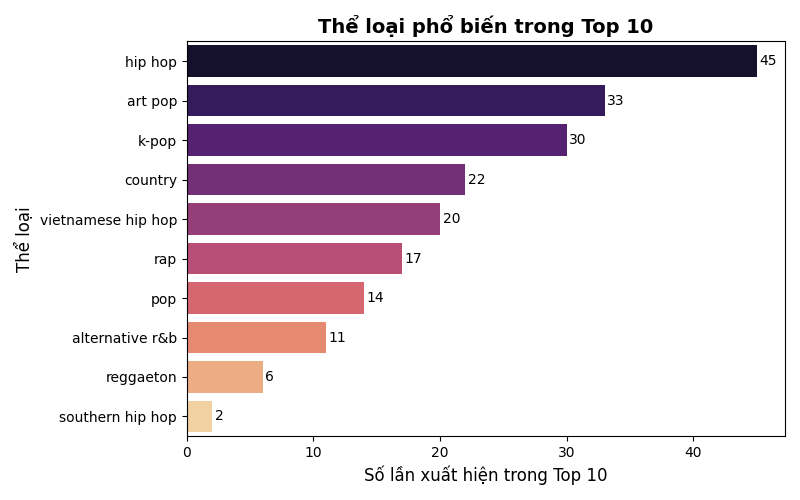
\includegraphics[width=1\textwidth]{../graphics/data3/Output/step4/top10_genres.png}
%         \caption{Top 10 thể loại âm nhạc phổ biến nhất trong BXH Billboard Hot 100.}
%         \label{fig:top10_genres}
%     \end{figure}
    
%     Biểu đồ cho thấy \textbf{Hip Hop} là thể loại thống trị, xuất hiện tới 45 lần trong Top 10, tiếp theo là \textbf{Art Pop} và \textbf{K-pop} với lần lượt 33 và 30 lần. Các thể loại như \textbf{Country}, \textbf{Vietnamese Hip Hop}, \textbf{Rap} và \textbf{Pop} cũng giữ vị trí quan trọng nhưng ít xuất hiện hơn.  
    
%     Điều này phản ánh sự đa dạng trong thị hiếu âm nhạc: Hip Hop và Pop vẫn giữ vai trò chủ đạo, nhưng những làn sóng mới như K-pop và Vietnamese Hip Hop đang có sự bứt phá mạnh mẽ, đóng góp đáng kể vào thị trường quốc tế. Ngoài ra, sự xuất hiện của thể loại nhỏ như \textbf{Southern Hip Hop} cho thấy một số “ngách” âm nhạc vẫn có thể vươn lên Top 10 trong những giai đoạn đặc biệt.


%     \item \textbf{Top nghệ sĩ trong Top 10}
%     \begin{itemize}
%         \item Nhóm theo nghệ sĩ, đếm số lượng ca khúc vào Top 10.
%         \item Xếp hạng Top 10 nghệ sĩ có nhiều hit nhất.
%     \end{itemize}
    
%     \begin{figure}[H]
%         \centering
%         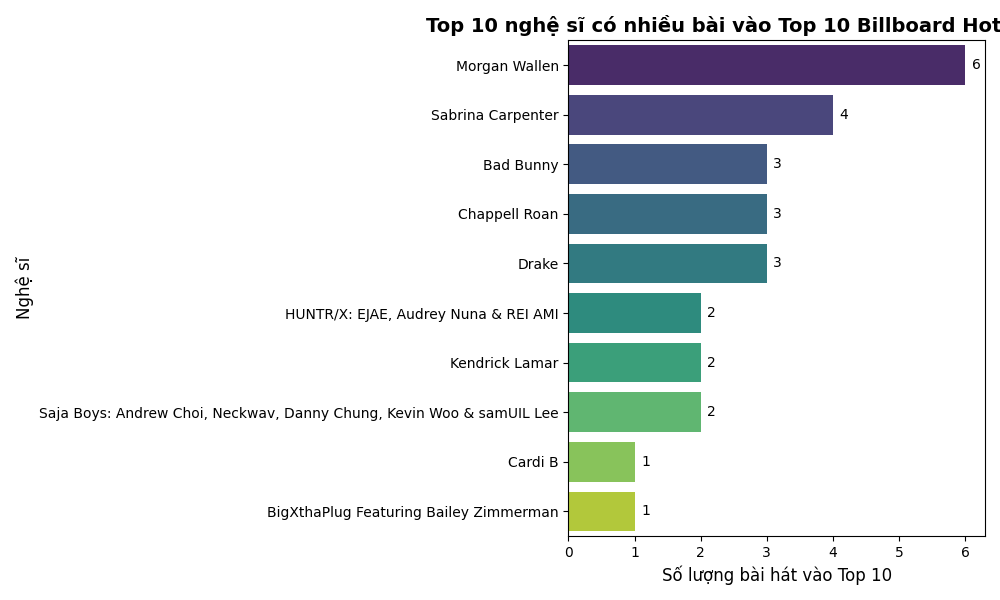
\includegraphics[width=0.9\textwidth]{../graphics/data3/Output/step4/top_artists_top10.png}
%         \caption{Top 10 nghệ sĩ có nhiều ca khúc lọt vào Top 10 Billboard Hot 100 năm 2025.}
%         \label{fig:top_artists}
%     \end{figure}
    
%     Biểu đồ cho thấy \textbf{Morgan Wallen} dẫn đầu với 6 ca khúc vào Top 10, 
%     khẳng định vị thế vững chắc trên thị trường âm nhạc năm 2025.  
%     Theo sau là \textbf{Sabrina Carpenter} với 4 ca khúc, trong khi các tên tuổi đình đám như  \textbf{Bad Bunny}, \textbf{Chappell Roan}, \textbf{Drake} đều có 3 bài lọt Top 10.  
    
%     Ngoài ra, nhiều nghệ sĩ khác như \textbf{Kendrick Lamar}, nhóm \textbf{HUNTR/X}, hay các nhóm hợp tác đa nghệ sĩ (\textbf{Saja Boys}) cũng góp mặt với 2 ca khúc. Các nghệ sĩ nổi tiếng như \textbf{Cardi B} hay \textbf{Bailey Zimmerman} tuy chỉ có 1 ca khúc vào Top 10 nhưng vẫn cho thấy sức ảnh hưởng nhất định.  
    
%     Điều này phản ánh rằng năm 2025 không chỉ có các tên tuổi kỳ cựu (Drake, Bad Bunny, Cardi B) mà còn chứng kiến sự vươn lên mạnh mẽ của những gương mặt mới (Chappell Roan, Sabrina Carpenter), làm đa dạng bức tranh thị trường âm nhạc toàn cầu.
    

%     \item \textbf{So sánh audio features theo mùa}
%     \begin{itemize}
%         \item Tính trung bình \texttt{danceability}, \texttt{energy}, \texttt{valence} cho mỗi mùa (Spring, Summer, Fall, Winter).
%         \item Vẽ bar chart để so sánh sự khác biệt.
%     \end{itemize}
    
%     \begin{figure}[H]
%         \centering
%         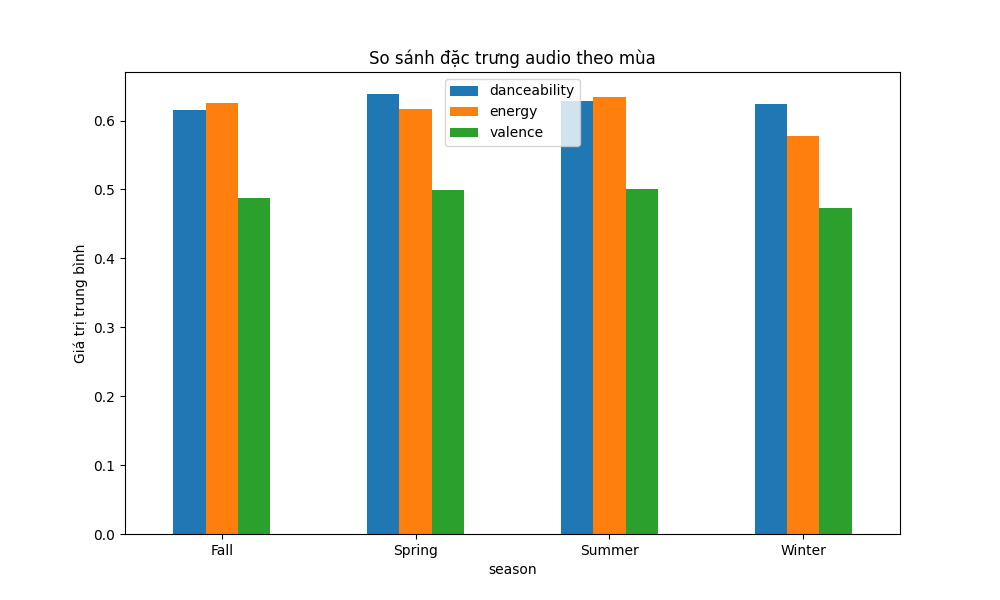
\includegraphics[width=0.8\textwidth]{../graphics/data3/Output/step4/season_features.png}
%         \caption{So sánh giá trị trung bình của các audio features theo mùa.}
%         \label{fig:season_features}
%     \end{figure}
    
%     Biểu đồ cho thấy có sự khác biệt nhẹ về đặc trưng âm nhạc giữa các mùa:  
%     \begin{itemize}
%         \item \textbf{Spring} và \textbf{Summer} có mức \texttt{danceability} và \texttt{energy} cao nhất, phản ánh xu hướng nghe nhạc sôi động, dễ nhảy trong mùa lễ hội và du lịch.  
%         \item \textbf{Fall} duy trì năng lượng cao nhưng \texttt{valence} thấp hơn, gợi ý sự xuất hiện nhiều hơn của các ca khúc buồn/ballad.  
%         \item \textbf{Winter} có \texttt{energy} và \texttt{valence} thấp nhất, cho thấy thiên hướng âm nhạc trầm lắng, sâu lắng phù hợp không khí cuối năm.  
%     \end{itemize}
    
%     Điều này chứng minh yếu tố \textbf{mùa vụ} có tác động đến thị hiếu nghe nhạc:  mùa Hè và Xuân ưu tiên nhạc sôi động, trong khi Thu và Đông phổ biến nhạc trữ tình, chậm rãi hơn.
    

%     \item \textbf{Mối quan hệ Longevity và Peak Rank}
%     \begin{itemize}
%         \item Vẽ scatter plot kèm regression line giữa \texttt{weeks\_on\_chart\_total} và \texttt{peak\_rank}.
%         \item Đánh giá mối liên hệ giữa thứ hạng cao nhất và tuổi thọ bài hát.
%     \end{itemize}
    
%     \begin{figure}[H]
%         \centering
%         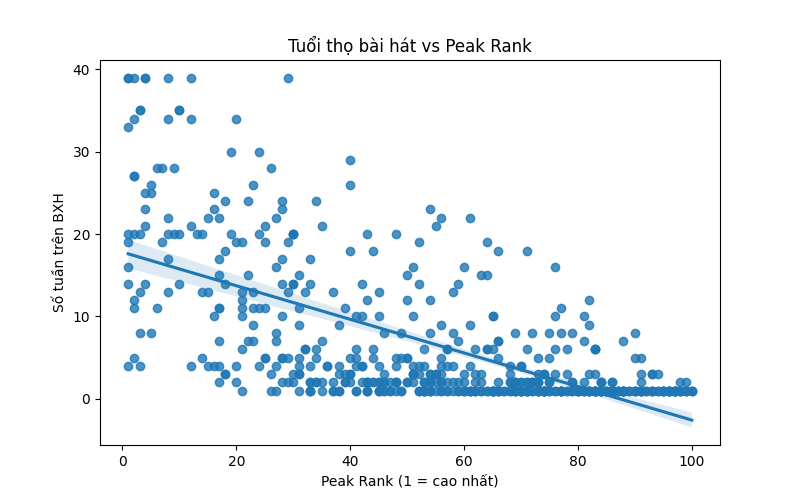
\includegraphics[width=0.8\textwidth]{../graphics/data3/Output/step4/longevity_vs_peak.png}
%         \caption{Mối quan hệ giữa Peak Rank và số tuần tồn tại trên BXH.}
%         \label{fig:longevity_vs_peak}
%     \end{figure}
    
%     Biểu đồ cho thấy có mối quan hệ nghịch giữa \textbf{Peak Rank} và \textbf{tuổi thọ bài hát} trên BXH.  
%     Cụ thể:  
%     \begin{itemize}
%         \item Những ca khúc đạt \texttt{peak\_rank} cao (từ 1–10) có xu hướng tồn tại nhiều tuần hơn trên BXH, thậm chí một số bài trụ vững hơn 30 tuần.  
%         \item Ngược lại, những bài chỉ đạt peak ở vị trí thấp (trên 50) thường rời BXH sau vài tuần ngắn ngủi.  
%         \item Regression line minh họa xu hướng này một cách rõ rệt: càng đạt vị trí cao, tuổi thọ trên BXH càng dài.  
%     \end{itemize}
    
%     Điều này khẳng định rằng: \textbf{vị trí đỉnh cao nhất mà bài hát từng đạt được là một chỉ báo quan trọng cho sự bền vững của nó trên thị trường}. 
%     Những bản hit lớn không chỉ leo lên Top 1 mà còn duy trì sức hút lâu dài, 
%     trong khi các bài có thứ hạng trung bình khó giữ chân khán giả trong nhiều tuần.

% \end{enumerate}

% \subsubsection{Kết quả và Ý nghĩa}

%     \textbf{Mục tiêu bài toán} \\
    
%     - Mục tiêu là xây dựng một \textbf{pipeline phân tích dữ liệu âm nhạc hoàn chỉnh}, giúp phát hiện các xu hướng nổi bật về hit songs, thể loại, nghệ sĩ, yếu tố mùa vụ và hành vi của thị trường. \\
    
%     \textbf{Kết quả đạt được} \\
    
%     \begin{itemize}
%         \item Hoàn thiện pipeline tự động với 4 bước: 
%         \textit{(i) Thu thập dữ liệu}, \textit{(ii) Làm sạch dữ liệu}, 
%         \textit{(iii) Tạo đặc trưng}, \textit{(iv) Phân tích xu hướng}.
%         \item Bổ sung các đặc trưng quan trọng (audio features, genres, track-level, artist-based, time-based), 
%         làm cho dữ liệu đa chiều và giàu ý nghĩa hơn.
%         \item Thực hiện EDA và trực quan hóa để đánh giá chất lượng dữ liệu, phát hiện vấn đề và xử lý kịp thời.
%         \item Một số insight chính: 
%         \begin{itemize}
%             \item Các hit chủ yếu tập trung ở \textbf{Hip-hop, Pop, K-pop, Country}.  
%             \item Nghệ sĩ có nhiều hợp tác thường xuất hiện dày đặc trong Top 10.  
%             \item Ca khúc đạt \texttt{peak rank} cao (Top 1–5) thường có tuổi thọ lâu hơn trên BXH.  
%             \item Yếu tố mùa vụ ảnh hưởng đến đặc trưng nhạc: Hè/Xuân thiên về nhạc sôi động (danceability, energy cao), 
%             Thu/Đông phổ biến ballad trữ tình với valence thấp.  
%         \end{itemize}
%     \end{itemize}
    
%     \textbf{Ý nghĩa} \\
    
%     - Bộ dữ liệu sau xử lý không chỉ phản ánh thứ hạng, mà còn lý giải được \textit{nguyên nhân thành công của một ca khúc} và \textit{xu hướng vận động của thị trường âm nhạc Mỹ}.  
%     - Pipeline này có thể mở rộng sang các năm khác hoặc thị trường khác, 
%     làm cơ sở cho phân tích so sánh xuyên quốc gia và ứng dụng trong \textbf{dự báo (predictive analytics)} về khả năng thành công của các ca khúc trong tương lai.  


% ===============================
\subsection{Nguồn 3: Billboard Hot 100}
\subsubsection{Giới thiệu dữ liệu}
    
    \textbf{Bối cảnh} \\
    
    - Từ năm 2025, Spotify đã ngừng công khai dữ liệu bảng xếp hạng \textbf{Global Top 200} hằng tuần. Điều này khiến việc thu thập dữ liệu gốc phục vụ cho phân tích trở nên khó khăn nếu chỉ dựa vào nguồn chính thức từ Spotify. \\
    
    - Để khắc phục hạn chế này, nhóm lựa chọn sử dụng \textbf{Billboard Hot 100} 
    làm nguồn dữ liệu thay thế. Đây là bảng xếp hạng uy tín, được cập nhật hằng tuần vào Chủ Nhật, phản ánh mức độ phổ biến của các ca khúc trên thị trường âm nhạc \textbf{Mỹ} và có sức ảnh hưởng toàn cầu. \\
    
    \textbf{Dữ liệu thu thập ban đầu} \\
    
    - Pipeline được xây dựng bằng Python, sử dụng thư viện \texttt{billboard} để tự động tải danh sách \textbf{Top 100 ca khúc mỗi tuần trong năm 2025}. \\
    
    - Các trường thông tin thu được gồm:
    \begin{itemize}
        \item \texttt{week}: ngày Chủ Nhật của tuần (chuẩn hóa mốc thời gian).
        \item \texttt{rank}: thứ hạng của bài hát trong tuần.
        \item \texttt{title}: tên bài hát.
        \item \texttt{artist}: nghệ sĩ thể hiện chính.
    \end{itemize}
    
    - Bộ dữ liệu này được lưu trữ ban đầu trong tệp, làm nền tảng cho các bước \textbf{bổ sung dữ liệu (enrichment)} ở giai đoạn sau. \\
    
    \textbf{Hạn chế của dữ liệu gốc} \\
    
    - Billboard chỉ cung cấp \textbf{thông tin xếp hạng và metadata cơ bản} (tựa đề, nghệ sĩ), chưa có định danh duy nhất để liên kết với dữ liệu ngoài. \\
    
    - Hoàn toàn thiếu vắng \textbf{đặc trưng âm thanh (audio features)} 
    và \textbf{thể loại (genres)} – trong khi đây lại là các yếu tố then chốt để phân tích sâu hơn về “công thức tạo hit” và “xu hướng thể loại theo thời gian”. \\

    

% =========================
\subsubsection{Thu thập và bổ sung dữ liệu }

\textbf{Giải pháp từng bước} 

\begin{enumerate}
    \item \textbf{Thu thập Billboard Hot 100}
    \begin{itemize}
        \item Sinh danh sách ngày Chủ Nhật trong năm 2025 và tải dữ liệu xếp hạng Hot 100 cho từng tuần. 
        \item \textbf{Kết quả:} dữ liệu gốc đã có thứ hạng bài hát theo tuần nhưng chưa đủ thông tin để phân tích chuyên sâu.
    \end{itemize}

    \item \textbf{Tìm Spotify track ID}
    \begin{itemize}
        \item Với mỗi cặp \texttt{(title, artist)} từ Billboard, gọi \textbf{Spotify Search API} để tìm \texttt{spotify\_id}. 
        \item  \textbf{Kết quả:} bổ sung khóa định danh duy nhất giúp liên kết với các API khác.
    \end{itemize}

    \item \textbf{Lấy audio features từ ReccoBeats}
    \begin{itemize}
        \item Gọi \textbf{ReccoBeats API} để lấy các đặc trưng âm nhạc: \texttt{danceability, energy, tempo, valence, speechiness, acousticness, instrumentalness, liveness, loudness, key, mode}.
        \item Do API giới hạn batch, pipeline được thiết kế để chia nhỏ các request (\texttt{BATCH\_SIZE = 30}). 
        \item \textbf{Kết quả:} dataset đã mô tả được ``chất âm'' của từng bài hát.
    \end{itemize}

    \item \textbf{Lấy genres từ Spotify API}
    \begin{itemize}
        \item Sử dụng \texttt{spotify\_id} để gọi endpoint \texttt{track/artist} nhằm lấy thể loại (genres) của nghệ sĩ chính.
        \item Nếu genres trống thì gán \texttt{NaN}.
        \item  \textbf{Kết quả:} dataset cuối cùng đã có thêm nhãn \textbf{thể loại âm nhạc} cho từng ca khúc.
    \end{itemize}


    
\end{enumerate}


% ==========================
    \subsubsection{Phân tích dữ liệu ban đầu}
    
    \textbf{Lý do} 
    
    - Sau khi đã bổ sung dữ liệu từ nhiều nguồn khác nhau, cần tiến hành phân tích dữ liệu ban đầu (Exploratory Data Analysis – EDA) 
    để hiểu rõ cấu trúc, chất lượng cũng như các vấn đề tiềm ẩn trước khi bước vào giai đoạn làm sạch và trích xuất đặc trưng. \\
    
    \textbf{Giải pháp} 
    
    \begin{enumerate}[label=\arabic*]
        \item \textbf{Tổng quan dữ liệu}
        \begin{itemize}
            \item Thống kê số dòng, số cột, tên các trường dữ liệu.
            \item Kiểm tra kiểu dữ liệu, số lượng giá trị bị thiếu (Null), số dòng trùng lặp.
            \item Tính toán các thống kê mô tả cơ bản cho dữ liệu số.
    \end{itemize}
     Số dòng: 3900, Số cột: 17
    \begin{longtable}{|>{\raggedright\arraybackslash}p{2.8cm}|
                          >{\raggedright\arraybackslash}p{2cm}|
                          >{\raggedright\arraybackslash}p{6cm}|
                          >{\raggedright\arraybackslash}p{5cm}|}
        \hline
        \textbf{Column} & \textbf{DataType} & \textbf{Meaning} & \textbf{How to Use} \\ \hline
        \endfirsthead
        
        \hline
        \textbf{Column} & \textbf{DataType} & \textbf{Meaning} & \textbf{How to Use} \\ \hline
        \endhead
        
        week & object & Ngày Chủ Nhật của tuần trong BXH Billboard (YYYY-MM-DD). & Mốc thời gian để phân tích xu hướng theo tuần. \\ \hline
        rank & int64 & Thứ hạng bài hát (1 = cao nhất, 100 = thấp nhất). & Phân tích Top 10/50, đo độ bền hạng, vẽ timeline. \\ \hline
        title & object & Tên bài hát. & Hiển thị trên dashboard, kết hợp với week để vẽ xu hướng. \\ \hline
        artist & object & Tên nghệ sĩ chính. & Phân tích Top Artist, số lần vào BXH, xu hướng hợp tác. \\ \hline
        spotify\_id & object & ID duy nhất của track trên Spotify. & Làm khóa để join với Spotify API/ReccoBeats. \\ \hline
        danceability & float64 & Mức độ dễ nhảy (0–1). & Đặc trưng hit songs, cao trong Pop/Dance. \\ \hline
        energy & float64 & Độ “năng lượng” của bài hát (0–1). & So sánh hit vs non-hit, nhận diện nhạc sôi động. \\ \hline
        tempo & float64 & Nhịp độ bài hát (beats per minute – BPM) & Phân tích BPM phổ biến trong các hit. \\ \hline
        valence & float64 & Mức độ tích cực/vui vẻ (0–1). & Phân biệt nhạc vui (valence cao) với ballad (thấp). \\ \hline
        speechiness & float64 & Mức độ giọng nói (0–1). & Cao trong Rap/Hip-hop, thấp trong Pop/Ballad. \\ \hline
        acousticness & float64 & Mức độ acoustic (0–1). & Ballad/Indie cao; Pop/EDM thấp. \\ \hline
        instrumentalness & float64 & Khả năng là nhạc không lời (0–1). & EDM/nhạc nền cao, Pop vocal thấp. \\ \hline
        liveness & float64 & Mức độ biểu diễn live (0–1). & Phát hiện bài hát thu live concert. \\ \hline
        loudness & float64 & Độ lớn trung bình (dB). & Kết hợp với energy để phân tích phong cách sản xuất. \\ \hline
        key & float64 & Tông nhạc (0–11). & Phân tích xu hướng tông nhạc ưa chuộng. \\ \hline
        mode & float64 & Thang âm: 1=Major, 0=Minor. & So sánh mood Major vs Minor. \\ \hline
        genre & object & Thể loại chính (Spotify API). & Nhóm xu hướng theo genre, Top genres theo rank/streams. \\ \hline
        
        \caption{Bảng mô tả dữ liệu }
        \label{tab:data_dictionary}
        \end{longtable}
    

    \item \textbf{Trực quan giá trị thiếu}
     \begin{itemize}
        \item Vẽ heatmap để quan sát sự phân bố các giá trị bị thiếu theo cột.
        \item Nhận diện các cột thiếu dữ liệu nhiều, cần xử lý trong bước làm sạch.
    \end{itemize}
    
    \begin{figure}[H] % dùng [H] để giữ hình tại đúng vị trí (cần \usepackage{float})
        \centering
        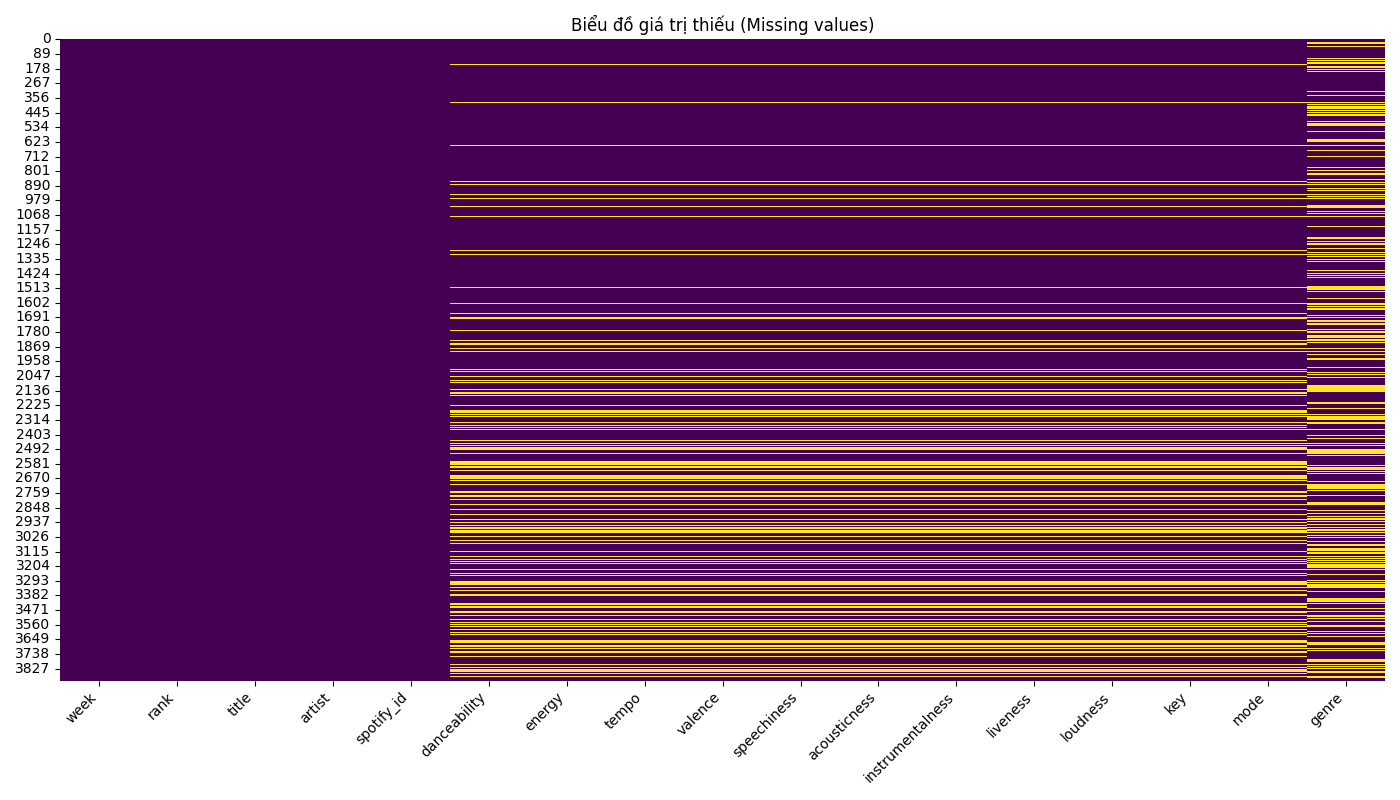
\includegraphics[width=1.0\textwidth]{../graphics/data3/Output/step1/missing_values.png}
        \caption{Biểu đồ heatmap thể hiện các giá trị thiếu trong dữ liệu}
        \label{fig:missing}
    \end{figure}
    Biểu đồ heatmap trên cho thấy một số cột dữ liệu xuất hiện nhiều giá trị thiếu (các vạch sáng). Cụ thể, các trường liên quan đến \texttt{audio features} (như \texttt{danceability}, \texttt{energy}, \texttt{tempo}, \texttt{valence}, \texttt{speechiness}, \texttt{acousticness}, \texttt{instrumentalness}, \texttt{liveness}, \texttt{loudness}) và trường \texttt{genre} có tỷ lệ thiếu khá cao. Điều này xuất phát từ việc Billboard chỉ cung cấp dữ liệu thứ hạng, tên bài hát và nghệ sĩ, trong khi các đặc trưng âm nhạc và thể loại phải được bổ sung từ API ngoài.  Việc trực quan hóa bằng heatmap giúp nhận diện nhanh các cột còn thiếu nhiều giá trị,từ đó đưa ra chiến lược xử lý hợp lý trong bước làm sạch dữ liệu.

    \item \textbf{Phân bố các thuộc tính âm nhạc}
    \begin{itemize}
        \item Vẽ histogram kèm KDE cho các thuộc tính quan trọng: \texttt{danceability}, \texttt{energy}, \texttt{tempo}, \texttt{valence}, 
        \texttt{speechiness}, \texttt{acousticness}, \texttt{instrumentalness}, \texttt{liveness}, \texttt{loudness}.
        \item Giúp hiểu rõ phân phối của từng đặc trưng.
        
         \begin{figure}[H] % dùng [H] để giữ hình tại đúng vị trí (cần \usepackage{float})
            \centering
            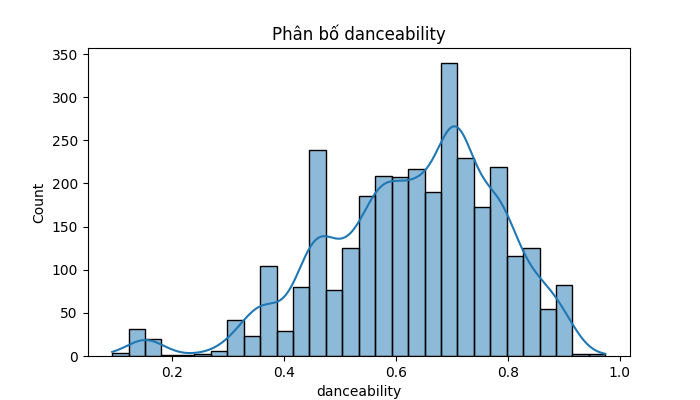
\includegraphics[width=1.0\textwidth]{../graphics/data3/Output/step1/danceability_distribution.png}
            \caption{Biểu đồ phân bố \texttt{danceability} của các bài hát.}
            \label{fig:missing}
        \end{figure}
    Biểu đồ trên cho thấy đa số các bài hát có giá trị \texttt{danceability} tập trung trong khoảng 0.5 -- 0.8. Điều này phản ánh rằng các ca khúc phổ biến trên thị trường âm nhạc toàn cầu thường có tiết tấu dễ nhảy, phù hợp với thị hiếu nghe nhạc của công chúng. Những bài hát có \texttt{danceability} quá thấp hoặc quá cao chỉ chiếm tỷ lệ nhỏ, cho thấy thị trường ưu tiên sự cân bằng giữa khả năng nhảy và tính giai điệu.
        
    \end{itemize}

    \item \textbf{Phân bố thể loại âm nhạc}
    \begin{itemize}
        \item Loại bỏ nhãn \texttt{NaN}, sau đó thống kê tần suất xuất hiện của các thể loại.
    \end{itemize}

    \begin{figure}[H] % dùng [H] để giữ hình tại đúng vị trí (cần \usepackage{float})
            \centering
            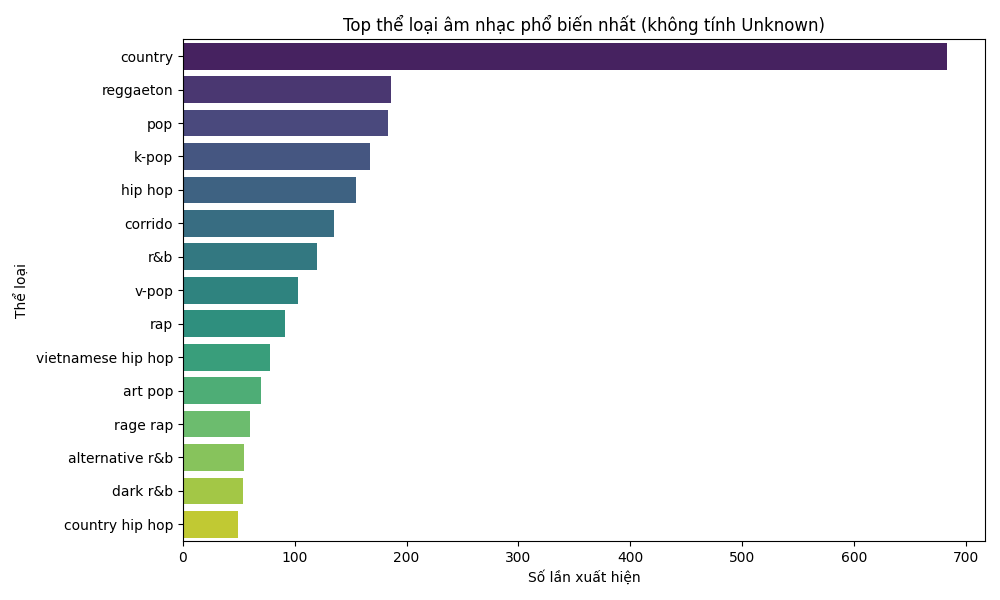
\includegraphics[width=1.0\textwidth]{../graphics/data3/Output/step1/genre_distribution.png}
            \caption{Top 15 thể loại âm nhạc phổ biến nhất .}
            \label{fig:missing}
    \end{figure}
    Biểu đồ trên cho thấy thể loại \textbf{Country} chiếm ưu thế vượt trội với gần 700 lần xuất hiện, cao hơn hẳn so với các thể loại còn lại. Các dòng nhạc như \textbf{Reggaeton}, \textbf{Pop}, \textbf{K-pop}, \textbf{Hip Hop} cũng nằm trong nhóm dẫn đầu, phản ánh xu hướng toàn cầu hiện nay. Đáng chú ý, \textbf{V-Pop} và \textbf{Vietnamese Hip Hop} cũng có sự hiện diện nhất định, cho thấy nhạc Việt đang dần khẳng định vị thế trong thị trường quốc tế. Sự phân bố này gợi ý rằng các doanh nghiệp và nghệ sĩ có thể ưu tiên đầu tư vào các thể loại đang thịnh hành như Country, Pop hay K-pop để tối ưu cơ hội tiếp cận khán giả rộng hơn.

    \item \textbf{Ma trận tương quan}
    \begin{itemize}
        \item Tính hệ số tương quan giữa các biến số.
        \item Phát hiện mối quan hệ mạnh.
        \begin{figure}[H] % dùng [H] để giữ hình tại đúng vị trí (cần \usepackage{float})
            \centering
            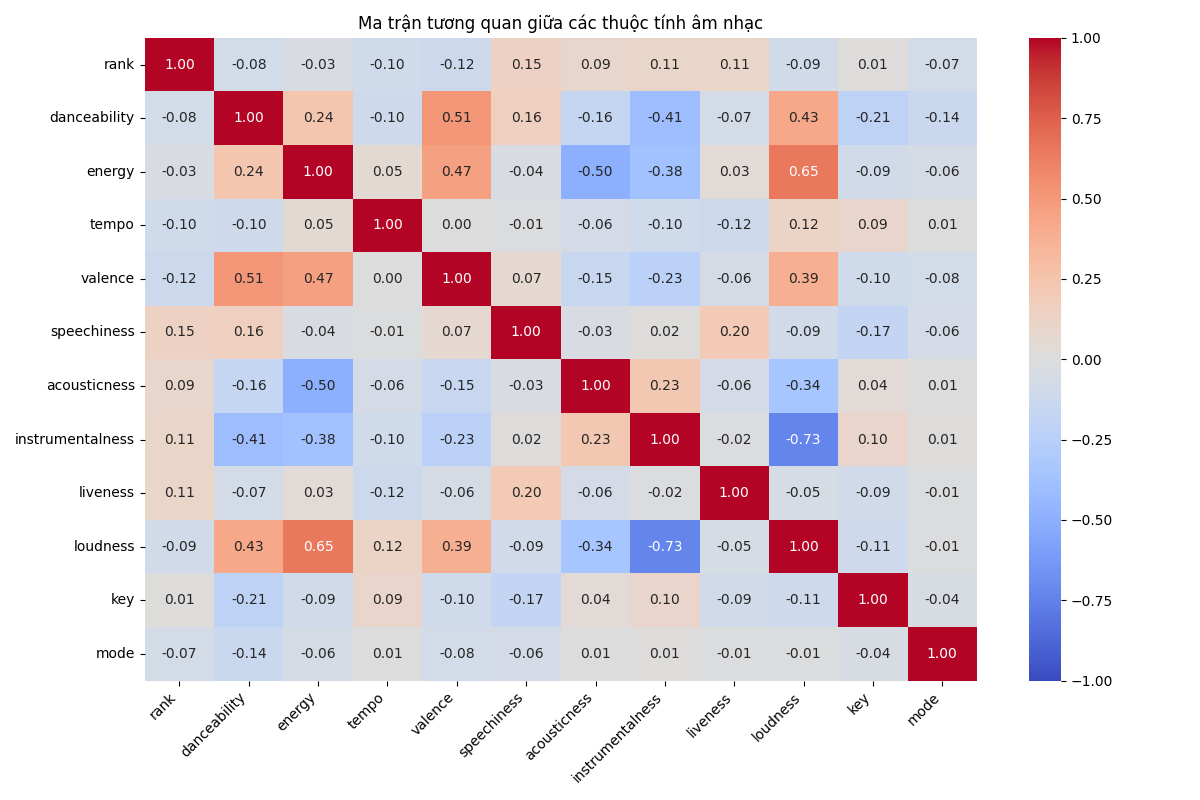
\includegraphics[width=1.0\textwidth]{../graphics/data3/Output/step1/correlation_matrix.png}
            \caption{Ma trận tương quan giữa các thuộc tính âm nhạc.}
            \label{fig:missing}
        \end{figure}
    Biểu đồ trên cho thấy một số mối quan hệ nổi bật giữa các đặc trưng âm nhạc. \textbf{Energy} có tương quan dương mạnh với \textbf{Loudness} (0.65), phản ánh rằng các bài hát có cường độ năng lượng cao thường đi kèm với âm lượng lớn. Ngược lại, \textbf{Acousticness} có tương quan âm với \textbf{Energy} (-0.50), cho thấy nhạc acoustic thường có mức năng lượng thấp. \textbf{Danceability} và \textbf{Valence} cũng có mối quan hệ dương (0.51), gợi ý rằng những ca khúc dễ nhảy thường mang lại cảm xúc tích cực. Những phát hiện này hỗ trợ việc lý giải tại sao một số thuộc tính đóng vai trò quan trọng trong việc tạo nên “công thức” của các bài hit toàn cầu.
    \end{itemize}
\end{enumerate}

\textbf{Kết quả / Ý nghĩa} 

\begin{itemize}
    \item Bộ dữ liệu đã được mô tả đầy đủ về cấu trúc và chất lượng, cung cấp cái nhìn tổng quan cần thiết trước khi làm sạch.
    \item Phát hiện được những vấn đề cần xử lý trong bước kế tiếp (missing values, dữ liệu trùng lặp, định dạng chưa thống nhất).
    \item Các insight sơ bộ: nhạc dễ nhảy (danceability) chiếm ưu thế, energy và loudness cao, acousticness thấp; 
    streams có quan hệ nghịch mạnh với rank. Đây là cơ sở định hướng cho bước làm sạch dữ liệu và xây dựng đặc trưng.
\end{itemize}
% =========================
\subsubsection{Làm sạch dữ liệu (Data Cleaning)}

\textbf{Lý do} \\

- Sau khi phân tích dữ liệu ban đầu mặc dù không có giá trị trùng lặp,nhưng nhận thấy còn tồn tại nhiều giá trị thiếu (missing values), một số cột chưa đúng kiểu dữ liệu.
- Nếu không xử lý, các vấn đề này sẽ gây sai lệch cho kết quả phân tích và trực quan hóa ở các bước tiếp theo. \\

\textbf{Giải pháp} \\

\begin{enumerate}[label=\arabic*]
    \item \textbf{Chuẩn hóa kiểu dữ liệu}
    \begin{itemize}
        \item Cột \texttt{week} được chuyển về định dạng \texttt{datetime}.
        \item Cột \texttt{rank} được ép kiểu về số nguyên \texttt{Int64}.
    \end{itemize}

    \item \textbf{Xử lý missing values}
    \begin{itemize}
        \item Với các cột số (\texttt{danceability}, \texttt{energy}, \texttt{tempo}, 
        \texttt{valence}, \texttt{speechiness}, \texttt{acousticness}, 
        \texttt{instrumentalness}, \texttt{liveness}, \texttt{loudness}, 
        \texttt{key}, \texttt{mode}): điền giá trị trung bình (mean).
        \item Với cột \texttt{genre}: điền giá trị mặc định là \texttt{Unknown} nếu bị thiếu.
    \end{itemize}

    \item \textbf{Đánh giá lại dữ liệu sau khi làm sạch}
    \begin{itemize}
        \item Sử dụng heatmap để trực quan hóa, xác nhận rằng toàn bộ giá trị thiếu đã được xử lý.
        \begin{figure}[H] % dùng [H] để giữ hình tại đúng vị trí (cần \usepackage{float})
            \centering
            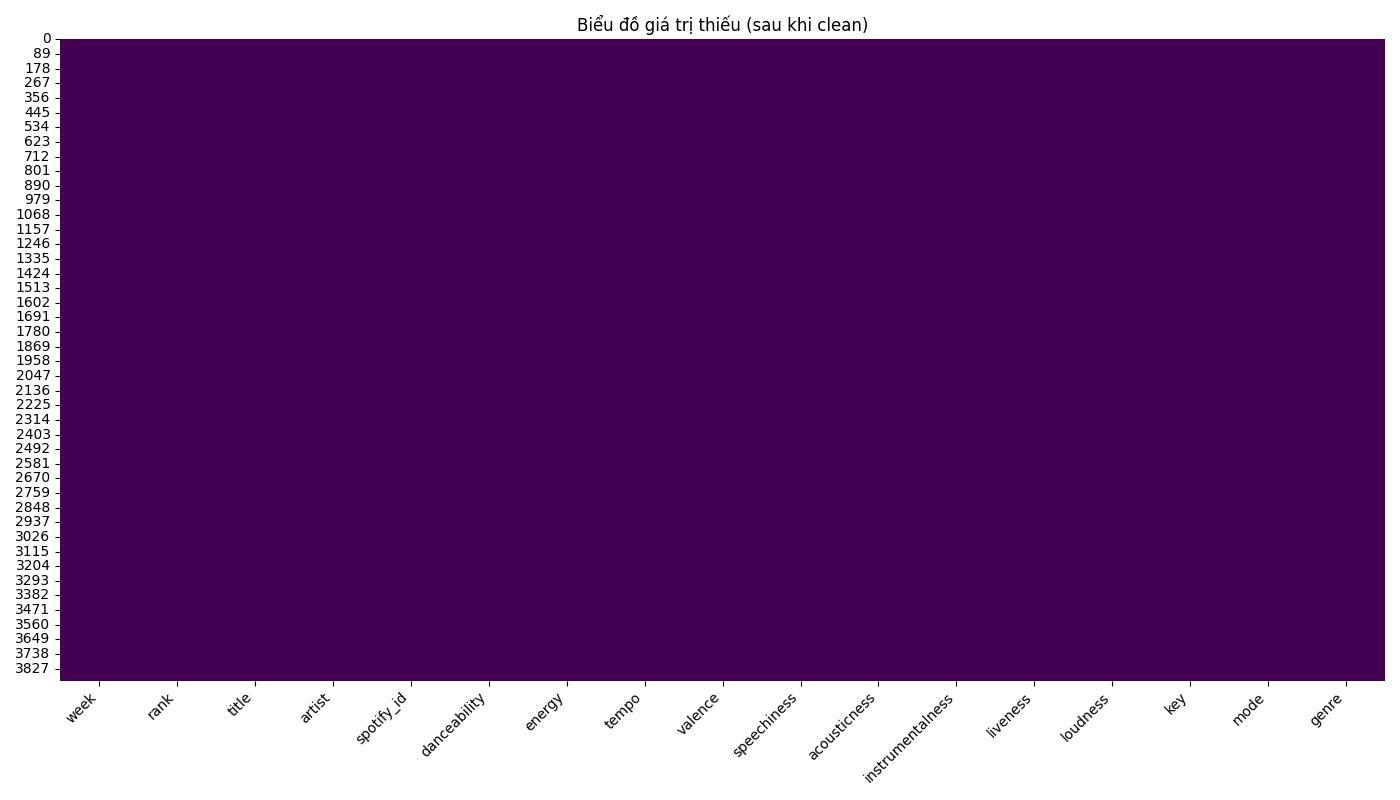
\includegraphics[width=1.0\textwidth]{../graphics/data3/Output/step2/missing_values_after_clean.png}
            \caption{Heatmap giá trị thiếu sau khi làm sạch dữ liệu.}
            \label{fig:missing}
        \end{figure}
        Biểu đồ trên cho thấy toàn bộ các cột dữ liệu đều đã được xử lý đầy đủ, 
    không còn giá trị thiếu. Điều này chứng minh quy trình làm sạch dữ liệu đã hoàn tất, tập dữ liệu đã đồng nhất và sẵn sàng cho các bước phân tích đặc trưng và xu hướng tiếp theo.

    \end{itemize}
\end{enumerate}

\textbf{Kết quả và Ý nghĩa} 

\begin{itemize}
    \item Bộ dữ liệu đã được chuẩn hóa và không còn giá trị thiếu.
    \item Các cột dữ liệu quan trọng đều ở định dạng chính xác, đảm bảo độ tin cậy cho các phép phân tích.
    \item Việc gán giá trị trung bình cho các cột số và điền \texttt{Unknown} cho thể loại 
    giúp giữ lại toàn bộ dữ liệu, không gây mất mát bản ghi.
    \item Dữ liệu sạch, đồng nhất, sẵn sàng cho bước tiếp theo: \textbf{Tạo đặc trưng (Feature Engineering)}.
\end{itemize}

% =========================
\subsubsection{Tạo đặc trưng (Feature Engineering)}

\textbf{Lý do} 
- Dữ liệu sau khi làm sạch vẫn chủ yếu mô tả thông tin cơ bản như thứ hạng, nghệ sĩ và đặc trưng âm nhạc. 
Tuy nhiên, để phân tích chuyên sâu hơn, cần có các biến phản ánh mức độ bền vững của bài hát trên BXH, 
đặc điểm nghệ sĩ (solo/hợp tác), cũng như yếu tố thời gian (mùa trong năm). 
- Việc tạo thêm đặc trưng mới sẽ giúp khám phá xu hướng ẩn và nâng cao giá trị phân tích. \\

\textbf{Giải pháp} 
\begin{enumerate}[label=\arabic*]
    \item \textbf{Đặc trưng theo bài hát (Track-level features)}
    \begin{itemize}
        \item \texttt{weeks\_on\_chart\_total}: tổng số tuần xuất hiện trên BXH.
        \item \texttt{weeks\_on\_chart\_cum}: số tuần tích lũy đến thời điểm hiện tại.
        \item \texttt{peak\_rank}: thứ hạng cao nhất mà bài hát đạt được.
        \item \texttt{avg\_rank}: thứ hạng trung bình của bài hát.
        \item \texttt{is\_top10}: 1 nếu bài hát lọt Top 10 trong tuần, ngược lại là 0.
        \item \texttt{is\_new}: 1 nếu đây là tuần đầu tiên xuất hiện trên BXH, ngược lại là 0.
    \end{itemize}

    \item \textbf{Đặc trưng theo nghệ sĩ (Artist-based features)}
    \begin{itemize}
        \item \texttt{is\_collab}: 1 nếu bài hát có sự hợp tác (nhiều nghệ sĩ, có “feat.”, “\&” hoặc dấu phẩy trong tên), 
        ngược lại là 0.
    \end{itemize}

    \item \textbf{Đặc trưng theo thời gian (Time-based features)}
    \begin{itemize}
        \item \texttt{season}: phân loại theo mùa (Spring, Summer, Fall, Winter) dựa trên tháng trong năm.
        \item Hỗ trợ phân tích yếu tố mùa vụ ảnh hưởng đến sự phổ biến của các thể loại nhạc.
    \end{itemize}
\end{enumerate}

\textbf{Kết quả và Ý nghĩa} 

\begin{itemize}
    \item Bộ dữ liệu sau khi thêm đặc trưng đã phản ánh đầy đủ hơn vòng đời của bài hát, đặc điểm nghệ sĩ và bối cảnh thời gian.
    \item Các đặc trưng như \texttt{peak\_rank}, \texttt{weeks\_on\_chart\_total} giúp đo lường mức độ bền vững của hit. 
    \item Đặc trưng \texttt{is\_collab} cho phép đánh giá vai trò của hợp tác nghệ sĩ trong việc tạo ra các ca khúc thành công.
    \item Đặc trưng \texttt{season} mở ra khả năng phân tích tác động của mùa vụ đến xu hướng nghe nhạc.
\end{itemize}

\begin{figure}[H]
    \centering
    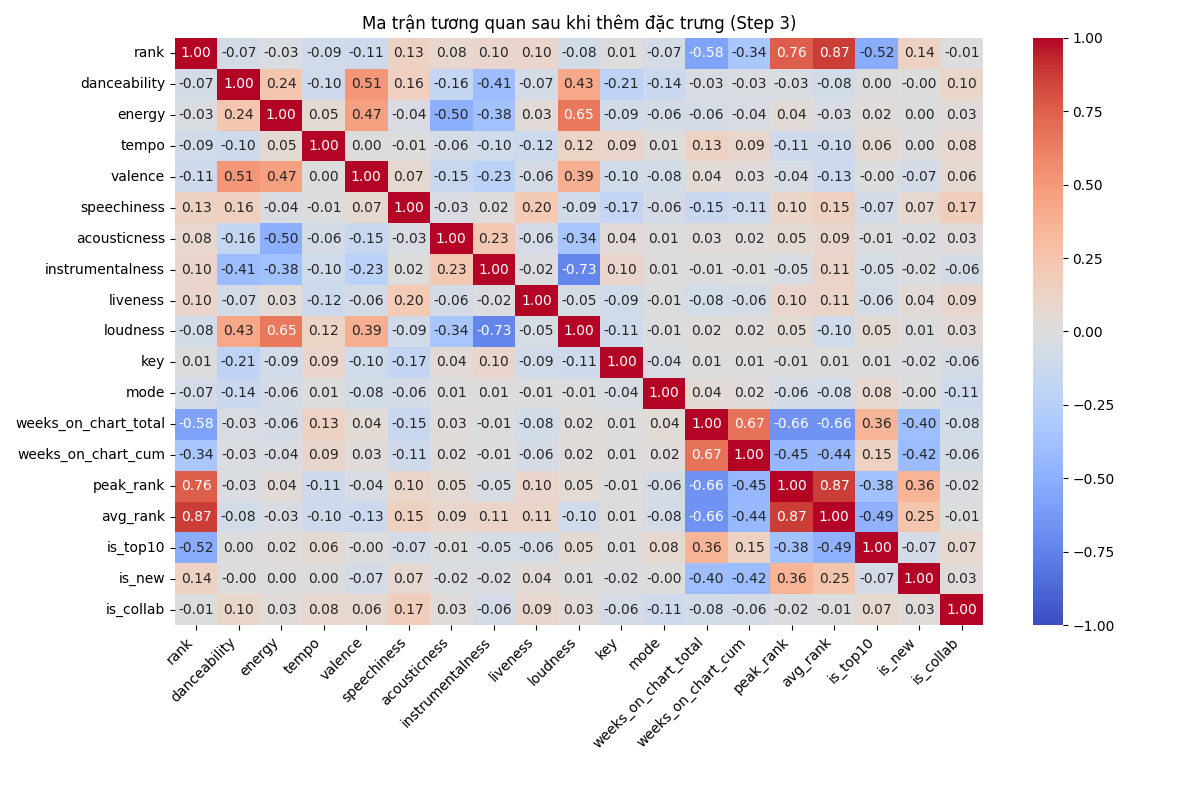
\includegraphics[width=1.0\textwidth]{../graphics/data3/Output/step3/correlation_matrix_step3.png}
    \caption{Ma trận tương quan sau khi thêm đặc trưng}
    \label{fig:corr_step3}
\end{figure}

Biểu đồ trên cho thấy các đặc trưng mới có mối quan hệ rõ rệt với các trường dữ liệu gốc: \texttt{weeks\_on\_chart\_total} và \texttt{weeks\_on\_chart\_cum} tương quan âm với \texttt{rank}, chứng tỏ các bài hát trụ hạng lâu thường có thứ hạng cao. \texttt{peak\_rank} và \texttt{avg\_rank} có tương quan mạnh với \texttt{rank}, khẳng định thứ hạng hàng tuần phản ánh hiệu suất tổng thể. 
Đặc trưng \texttt{is\_top10} cũng có quan hệ nghịch với \texttt{rank}, 
phù hợp với định nghĩa lọt Top 10. Trong khi đó, \texttt{is\_collab} và \texttt{is\_new} có tương quan yếu, nhưng vẫn là những yếu tố bổ sung quan trọng cho phân tích xu hướng và hành vi âm nhạc. 
% ==========================

\subsubsection{Phân tích xu hướng (Trend Analysis)}

\textbf{Bối cảnh} \\

Phần phân tích này tập trung vào dữ liệu \textbf{Billboard Hot 100 tại thị trường Mỹ năm 2025}, được bổ sung thông tin từ Spotify API và ReccoBeats. 
Do đặc thù Billboard Hot 100 phản ánh riêng thị trường Mỹ, các insight thu được sẽ cho thấy rõ xu hướng âm nhạc chủ đạo tại Mỹ thay vì toàn cầu.

\textbf{Lý do} \\

- Sau khi dữ liệu đã được làm sạch và bổ sung đặc trưng, bước tiếp theo là tiến hành phân tích xu hướng. 
- Mục tiêu nhằm phát hiện các mẫu hành vi nổi bật: cách bài hát mới xuất hiện, độ bền hit, thể loại phổ biến trong Top 10, vai trò của nghệ sĩ, yếu tố mùa vụ và mối quan hệ giữa độ bền (longevity) và vị trí cao nhất (peak rank). \\

\textbf{Giải pháp} \\

\begin{enumerate}[label=\arabic*]
    \item \textbf{Xu hướng bài hát mới theo thời gian}
    \begin{itemize}
        \item Đếm số lượng \texttt{is\_new} theo tuần để theo dõi số lượng bài hát mới gia nhập BXH.
        \item Trực quan bằng line chart cho thấy tuần nào có nhiều ca khúc debut nhất.
    \end{itemize}
    \begin{figure}[H]
        \centering
        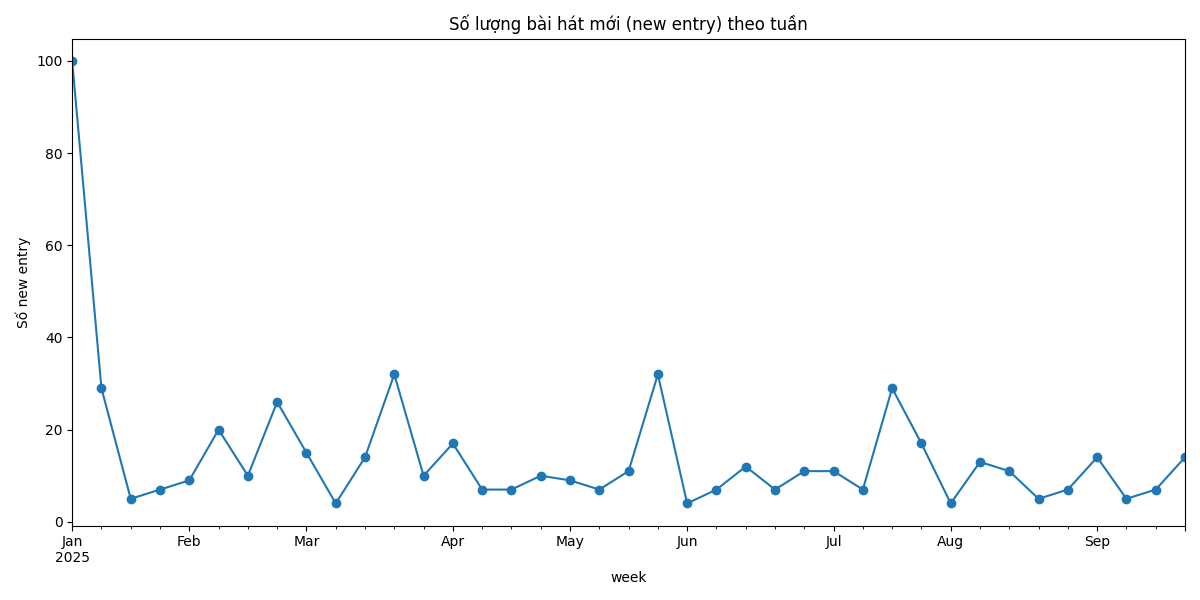
\includegraphics[width=1.0\textwidth]{../graphics/data3/Output/step4/new_entry_trend.png}
        \caption{Số lượng bài hát mới (new entry) theo tuần trong năm 2025.}
        \label{fig:new_entry_trend}
    \end{figure}
    Biểu đồ cho thấy trong tuần đầu tiên của năm 2025 có hơn 100 bài hát mới xuất hiện trên BXH Billboard Hot 100 (hiện tượng “reset” đầu năm). Sau đó, số lượng new entry giảm mạnh và dao động quanh mức 5–30 bài mỗi tuần.  Một số tuần có đột biến tăng (ví dụ cuối tháng 3, tháng 6, tháng 8), thường trùng với các đợt phát hành album lớn hoặc cao điểm mùa lễ hội. Điều này phản ánh tính cạnh tranh của thị trường âm nhạc.

    \item \textbf{Phân phối độ bền (longevity)}
    \begin{itemize}
        \item Vẽ histogram số tuần một bài hát tồn tại trên BXH.
        \item Giúp phân biệt hit “chớp nhoáng” và hit bền vững.
    \end{itemize}
    
    \begin{figure}[H]
        \centering
        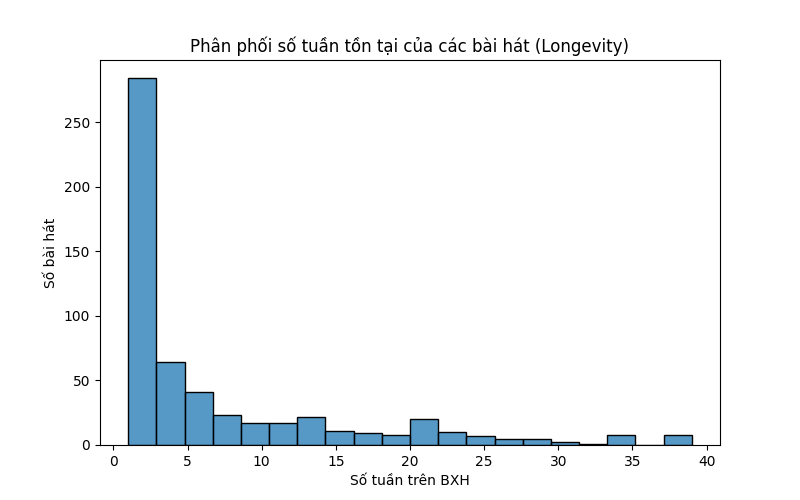
\includegraphics[width=1\textwidth]{../graphics/data3/Output/step4/hit_longevity.png}
        \caption{Phân phối số tuần tồn tại của các bài hát trên Billboard Hot 100.}
        \label{fig:hit_longevity}
    \end{figure}
    
    Biểu đồ cho thấy phần lớn các bài hát chỉ xuất hiện trên BXH trong thời gian ngắn (khoảng 1–3 tuần), phản ánh đặc trưng cạnh tranh khốc liệt của thị trường âm nhạc.  Tuy nhiên, vẫn có một nhóm nhỏ ca khúc duy trì được vị trí lâu dài (trên 20–30 tuần), được xem là những “hit bền vững” có sức hút mạnh mẽ.  
    Kết quả này gợi ý rằng việc duy trì vị trí lâu dài trên BXH khó khăn hơn nhiều so với việc “đột phá” vào BXH ở tuần đầu tiên, và có thể phụ thuộc vào các yếu tố như độ nổi tiếng của nghệ sĩ, chiến dịch quảng bá, cũng như đặc điểm âm nhạc (energy, danceability, valence).
    

   \item \textbf{Timeline các hit đình đám}
    \begin{itemize}
        \item Chọn ra một số bài có \texttt{peak\_rank = 1}, vẽ line chart thứ hạng theo thời gian.
        \item Đảo ngược trục Y để thể hiện trực quan đường đi lên/xuống BXH.
    \end{itemize}
    
    \begin{figure}[H]
        \centering
        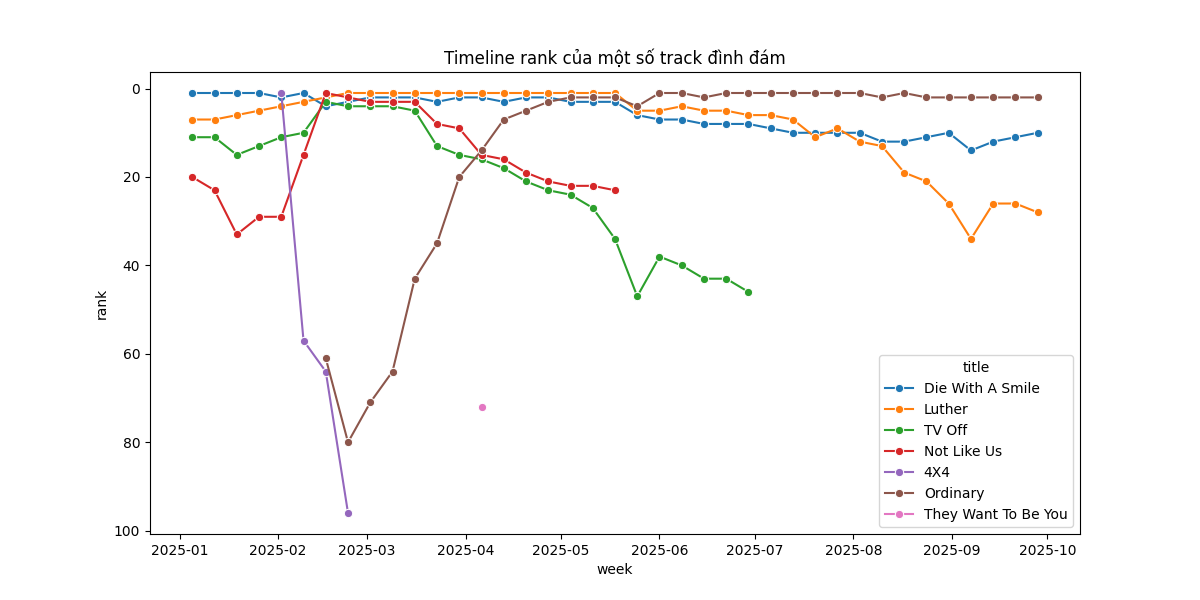
\includegraphics[width=1\textwidth]{../graphics/data3/Output/step4/track_timeline.png}
        \caption{Timeline thứ hạng của một số ca khúc đạt vị trí số 1 trên Billboard Hot 100.}
        \label{fig:track_timeline}
    \end{figure}
    
    Biểu đồ trên minh họa quá trình lên xuống hạng của một số bài hit nổi bật trong năm 2025. Có thể quan sát rằng:  
    \begin{itemize}
        \item Một số ca khúc như \textit{Die With A Smile}, \textit{Luther} giữ được vị trí cao trong thời gian dài, chứng tỏ sức hút ổn định và khả năng duy trì độ phổ biến.  
        \item Các bài như \textit{TV Off}, \textit{Not Like Us} nhanh chóng leo lên Top 1 nhưng tụt hạng mạnh sau vài tuần, thể hiện đặc điểm “bùng nổ ngắn hạn”.  
        \item Một số bài khác có quỹ đạo đi lên dần (ví dụ \textit{Ordinary}), cho thấy hiệu ứng lan tỏa muộn nhờ truyền thông hoặc viral.  
    \end{itemize}
    
    Điều này phản ánh sự đa dạng trong vòng đời của một hit: có ca khúc “one-hit wonder” chỉ thịnh hành trong thời gian ngắn, trong khi một số khác có khả năng trụ vững nhiều tháng liền nhờ nền tảng fanbase và chiến lược quảng bá hiệu quả.
    

    \item \textbf{Phân tích thể loại trong Top 10}
    \begin{itemize}
        \item Lọc các bài có \texttt{is\_top10 = 1}, loại bỏ \texttt{Unknown}.
        \item Đếm tần suất xuất hiện của từng thể loại → Top 10 genres.
    \end{itemize}
    
    \begin{figure}[H]
        \centering
        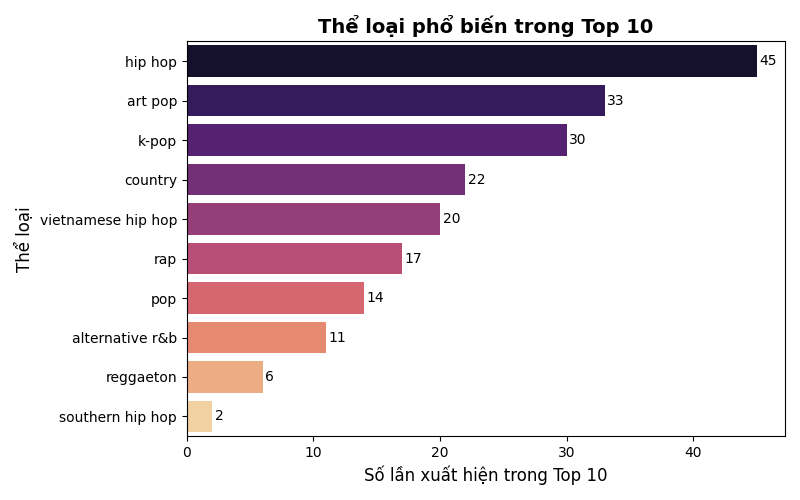
\includegraphics[width=1\textwidth]{../graphics/data3/Output/step4/top10_genres.png}
        \caption{Top 10 thể loại âm nhạc phổ biến nhất trong BXH Billboard Hot 100.}
        \label{fig:top10_genres}
    \end{figure}
    
    Biểu đồ cho thấy \textbf{Hip Hop} là thể loại thống trị, xuất hiện tới 45 lần trong Top 10, tiếp theo là \textbf{Art Pop} và \textbf{K-pop} với lần lượt 33 và 30 lần. Các thể loại như \textbf{Country}, \textbf{Vietnamese Hip Hop}, \textbf{Rap} và \textbf{Pop} cũng giữ vị trí quan trọng nhưng ít xuất hiện hơn.  
    
    Điều này phản ánh sự đa dạng trong thị hiếu âm nhạc: Hip Hop và Pop vẫn giữ vai trò chủ đạo, nhưng những làn sóng mới như K-pop và Vietnamese Hip Hop đang có sự bứt phá mạnh mẽ, đóng góp đáng kể vào thị trường quốc tế. Ngoài ra, sự xuất hiện của thể loại nhỏ như \textbf{Southern Hip Hop} cho thấy một số “ngách” âm nhạc vẫn có thể vươn lên Top 10 trong những giai đoạn đặc biệt.


    \item \textbf{Top nghệ sĩ trong Top 10}
    \begin{itemize}
        \item Nhóm theo nghệ sĩ, đếm số lượng ca khúc vào Top 10.
        \item Xếp hạng Top 10 nghệ sĩ có nhiều hit nhất.
    \end{itemize}
    
    \begin{figure}[H]
        \centering
        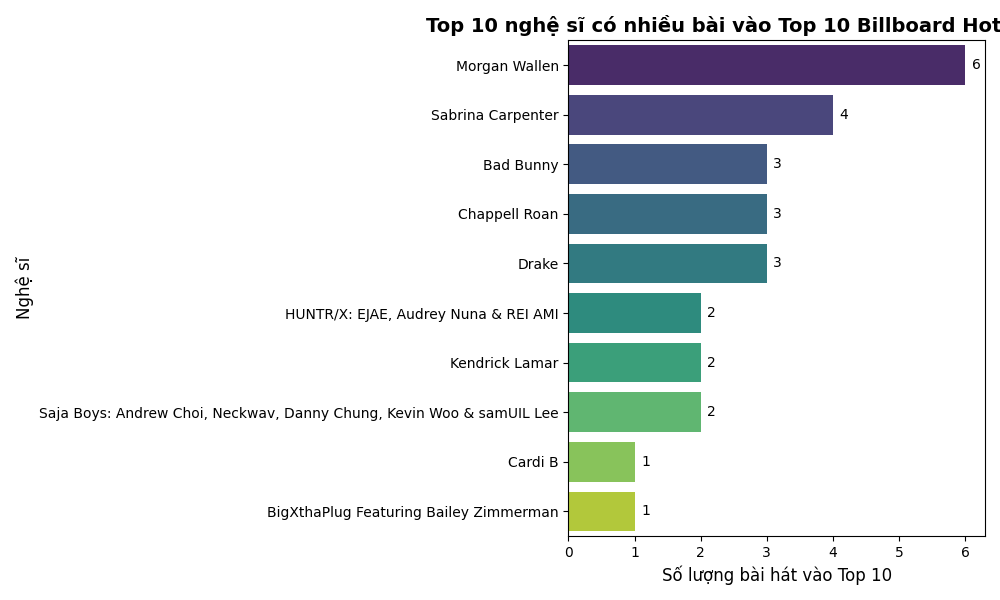
\includegraphics[width=0.9\textwidth]{../graphics/data3/Output/step4/top_artists_top10.png}
        \caption{Top 10 nghệ sĩ có nhiều ca khúc lọt vào Top 10 Billboard Hot 100 năm 2025.}
        \label{fig:top_artists}
    \end{figure}
    
    Biểu đồ cho thấy \textbf{Morgan Wallen} dẫn đầu với 6 ca khúc vào Top 10, 
    khẳng định vị thế vững chắc trên thị trường âm nhạc năm 2025.  
    Theo sau là \textbf{Sabrina Carpenter} với 4 ca khúc, trong khi các tên tuổi đình đám như  \textbf{Bad Bunny}, \textbf{Chappell Roan}, \textbf{Drake} đều có 3 bài lọt Top 10.  
    
    Ngoài ra, nhiều nghệ sĩ khác như \textbf{Kendrick Lamar}, nhóm \textbf{HUNTR/X}, hay các nhóm hợp tác đa nghệ sĩ (\textbf{Saja Boys}) cũng góp mặt với 2 ca khúc. Các nghệ sĩ nổi tiếng như \textbf{Cardi B} hay \textbf{Bailey Zimmerman} tuy chỉ có 1 ca khúc vào Top 10 nhưng vẫn cho thấy sức ảnh hưởng nhất định.  
    
    Điều này phản ánh rằng năm 2025 không chỉ có các tên tuổi kỳ cựu (Drake, Bad Bunny, Cardi B) mà còn chứng kiến sự vươn lên mạnh mẽ của những gương mặt mới (Chappell Roan, Sabrina Carpenter), làm đa dạng bức tranh thị trường âm nhạc toàn cầu.
    

    \item \textbf{So sánh audio features theo mùa}
    \begin{itemize}
        \item Tính trung bình \texttt{danceability}, \texttt{energy}, \texttt{valence} cho mỗi mùa (Spring, Summer, Fall, Winter).
        \item Vẽ bar chart để so sánh sự khác biệt.
    \end{itemize}
    
    \begin{figure}[H]
        \centering
        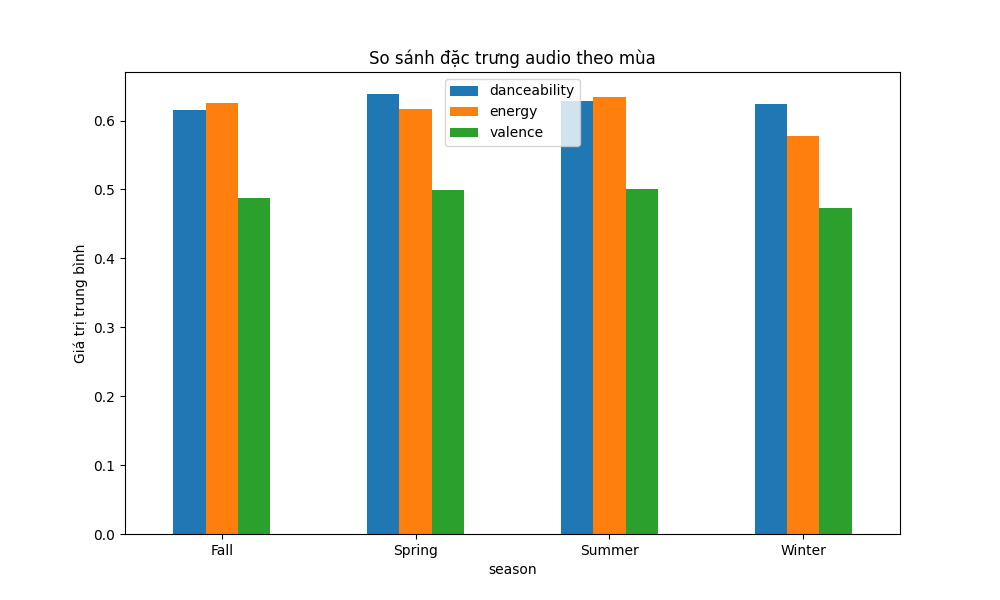
\includegraphics[width=0.8\textwidth]{../graphics/data3/Output/step4/season_features.png}
        \caption{So sánh giá trị trung bình của các audio features theo mùa.}
        \label{fig:season_features}
    \end{figure}
    
    Biểu đồ cho thấy có sự khác biệt nhẹ về đặc trưng âm nhạc giữa các mùa:  
    \begin{itemize}
        \item \textbf{Spring} và \textbf{Summer} có mức \texttt{danceability} và \texttt{energy} cao nhất, phản ánh xu hướng nghe nhạc sôi động, dễ nhảy trong mùa lễ hội và du lịch.  
        \item \textbf{Fall} duy trì năng lượng cao nhưng \texttt{valence} thấp hơn, gợi ý sự xuất hiện nhiều hơn của các ca khúc buồn/ballad.  
        \item \textbf{Winter} có \texttt{energy} và \texttt{valence} thấp nhất, cho thấy thiên hướng âm nhạc trầm lắng, sâu lắng phù hợp không khí cuối năm.  
    \end{itemize}
    
    Điều này chứng minh yếu tố \textbf{mùa vụ} có tác động đến thị hiếu nghe nhạc:  mùa Hè và Xuân ưu tiên nhạc sôi động, trong khi Thu và Đông phổ biến nhạc trữ tình, chậm rãi hơn.
    

    \item \textbf{Mối quan hệ Longevity và Peak Rank}
    \begin{itemize}
        \item Vẽ scatter plot kèm regression line giữa \texttt{weeks\_on\_chart\_total} và \texttt{peak\_rank}.
        \item Đánh giá mối liên hệ giữa thứ hạng cao nhất và tuổi thọ bài hát.
    \end{itemize}
    
    \begin{figure}[H]
        \centering
        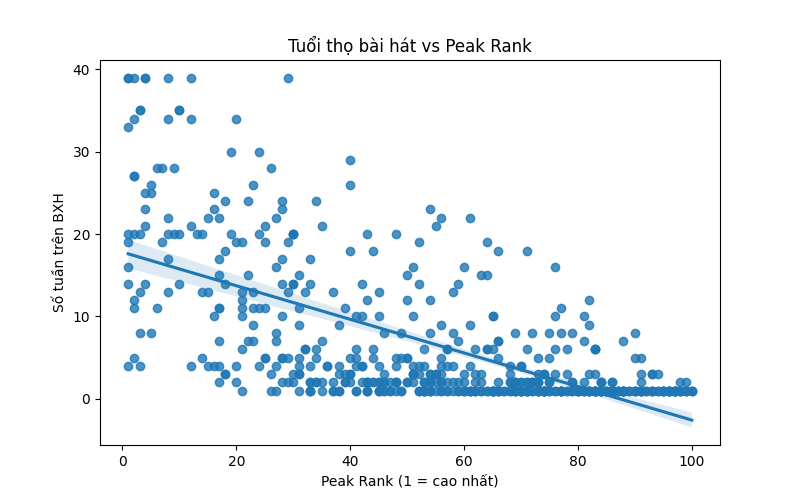
\includegraphics[width=0.8\textwidth]{../graphics/data3/Output/step4/longevity_vs_peak.png}
        \caption{Mối quan hệ giữa Peak Rank và số tuần tồn tại trên BXH.}
        \label{fig:longevity_vs_peak}
    \end{figure}
    
    Biểu đồ cho thấy có mối quan hệ nghịch giữa \textbf{Peak Rank} và \textbf{tuổi thọ bài hát} trên BXH.  
    Cụ thể:  
    \begin{itemize}
        \item Những ca khúc đạt \texttt{peak\_rank} cao (từ 1–10) có xu hướng tồn tại nhiều tuần hơn trên BXH, thậm chí một số bài trụ vững hơn 30 tuần.  
        \item Ngược lại, những bài chỉ đạt peak ở vị trí thấp (trên 50) thường rời BXH sau vài tuần ngắn ngủi.  
        \item Regression line minh họa xu hướng này một cách rõ rệt: càng đạt vị trí cao, tuổi thọ trên BXH càng dài.  
    \end{itemize}
    
    Điều này khẳng định rằng: \textbf{vị trí đỉnh cao nhất mà bài hát từng đạt được là một chỉ báo quan trọng cho sự bền vững của nó trên thị trường}. 
    Những bản hit lớn không chỉ leo lên Top 1 mà còn duy trì sức hút lâu dài, 
    trong khi các bài có thứ hạng trung bình khó giữ chân khán giả trong nhiều tuần.

\end{enumerate}

\subsubsection{Kết quả và Ý nghĩa}

    \textbf{Mục tiêu bài toán} \\
    
    - Mục tiêu là xây dựng một \textbf{pipeline phân tích dữ liệu âm nhạc hoàn chỉnh}, giúp phát hiện các xu hướng nổi bật về hit songs, thể loại, nghệ sĩ, yếu tố mùa vụ và hành vi của thị trường. \\
    
    \textbf{Kết quả đạt được} \\
    
    \begin{itemize}
        \item Hoàn thiện pipeline tự động với 4 bước: 
        \textit{(i) Thu thập dữ liệu}, \textit{(ii) Làm sạch dữ liệu}, 
        \textit{(iii) Tạo đặc trưng}, \textit{(iv) Phân tích xu hướng}.
        \item Bổ sung các đặc trưng quan trọng (audio features, genres, track-level, artist-based, time-based), 
        làm cho dữ liệu đa chiều và giàu ý nghĩa hơn.
        \item Thực hiện EDA và trực quan hóa để đánh giá chất lượng dữ liệu, phát hiện vấn đề và xử lý kịp thời.
        \item Một số insight chính: 
        \begin{itemize}
            \item Các hit chủ yếu tập trung ở \textbf{Hip-hop, Pop, K-pop, Country}.  
            \item Nghệ sĩ có nhiều hợp tác thường xuất hiện dày đặc trong Top 10.  
            \item Ca khúc đạt \texttt{peak rank} cao (Top 1–5) thường có tuổi thọ lâu hơn trên BXH.  
            \item Yếu tố mùa vụ ảnh hưởng đến đặc trưng nhạc: Hè/Xuân thiên về nhạc sôi động (danceability, energy cao), 
            Thu/Đông phổ biến ballad trữ tình với valence thấp.  
        \end{itemize}
    \end{itemize}
    
    \textbf{Ý nghĩa} \\
    
    - Bộ dữ liệu sau xử lý không chỉ phản ánh thứ hạng, mà còn lý giải được \textit{nguyên nhân thành công của một ca khúc} và \textit{xu hướng vận động của thị trường âm nhạc Mỹ}.  
    - Pipeline này có thể mở rộng sang các năm khác hoặc thị trường khác, 
    làm cơ sở cho phân tích so sánh xuyên quốc gia và ứng dụng trong \textbf{dự báo (predictive analytics)} về khả năng thành công của các ca khúc trong tương lai.  
